\documentclass[12pt, a4paper, hidelinks]{article}

\usepackage{graphicx}
\usepackage{hyperref}
\usepackage{xcolor}
\usepackage[english]{babel}
\usepackage[nottoc]{tocbibind}
\usepackage[utf8]{inputenc}
\usepackage[T1]{fontenc}
\usepackage[style=verbose,backend=biber,style=authoryear, citestyle=authoryear ]{biblatex}
\addbibresource{ref.bib} % The filename of the bibliography
\usepackage[left=2.5cm,right=2.5cm,top=2.5cm,bottom=2.5cm]{geometry}
\usepackage{acronym}
\usepackage{fancyhdr}
\pagestyle{fancy}
\usepackage{lipsum}
\usepackage{array, tabularx, booktabs} % For better tables
\usepackage{booktabs}
\usepackage{multirow}
\usepackage{longtable}
%\usepackage{listings} % Code environments
%\usepackage{lstautogobble}  % Fix relative indenting
%\usepackage{color}          % Code coloring
%\usepackage{zi4}            % Nice font
\usepackage{minted}
\usemintedstyle{tango}
\setminted{linenos, autogobble, bgcolor=gray!5}
\usepackage{cleveref}
\usepackage{titlesec}
\setlength{\marginparwidth}{2cm}
\usepackage{todonotes}
\usepackage[autostyle=true]{csquotes}
\usepackage{caption}

\iffalse

\definecolor{codegreen}{rgb}{0,0.6,0}
\definecolor{codegray}{rgb}{0.5,0.5,0.5}
\definecolor{backcolour}{gray}{0.95}
\definecolor{codeorange}{rgb}{0.8,0.5,0.2}

\lstdefinestyle{mystyle}{
    backgroundcolor=\color{backcolour},  
    commentstyle=\color{codegray},
    keywordstyle=\color{codeorange},
    numberstyle=\tiny\color{codegray},
    stringstyle=\color{codegreen},
    basicstyle=\ttfamily\footnotesize,
    breakatwhitespace=false,         
    breaklines=true,                 
    captionpos=b,                    
    keepspaces=true,                 
    numbers=left,                    
    numbersep=5pt,                  
    showspaces=false,                
    showstringspaces=false,
    showtabs=false,                  
    tabsize=2
}

%\lstset{style=mystyle}

\definecolor{bluekeywords}{rgb}{0.13, 0.13, 1}
\definecolor{greencomments}{rgb}{0, 0.5, 0}
\definecolor{redstrings}{rgb}{0.9, 0, 0}
\definecolor{graynumbers}{rgb}{0.5, 0.5, 0.5}

\usepackage{listings}
\lstset{
    autogobble,
    columns=fullflexible,
    showspaces=false,
    showtabs=false,
    breaklines=true,
    showstringspaces=false,
    breakatwhitespace=true,
    escapeinside={(*@}{@*)},
    commentstyle=\color{greencomments},
    keywordstyle=\color{bluekeywords},
    stringstyle=\color{redstrings},
    numberstyle=\color{graynumbers},
    basicstyle=\ttfamily\footnotesize,
    frame=l,
    framesep=12pt,
    xleftmargin=12pt,
    tabsize=4,
    captionpos=b
}

\fi

\titleformat{\section}[hang]{\huge\bfseries}{\thesection\hspace{20pt}}{0pt}{\huge\bfseries}
\graphicspath{{Figures/}{./}{Assets/}}

% --- document configuration ---

\newcommand{\thesistitle}{Profiling tree species classification with synthetic data and deep learning}  
\newcommand{\supervisor}{Dorothea Sommer} 
\newcommand{\authorname}{Hauke Kirchner}
%\newcommand{\university}{Georg-August-Universität Göttingen}
%\newcommand{\department}{Institute of Computer Science}
\newcommand{\thesistype}{Seminar Report}
%\newcommand{\matrikelnumber}{[Put your matrikel number here]}
\newcommand{\keywords}{} % Set keywords that describe your report

\hypersetup{pdftitle=\thesistitle} % Set the PDF's title to your title
\hypersetup{pdfauthor=\authorname} % Set the PDF's author to your name
\hypersetup{pdfkeywords=\keywords} % Set the PDF's keywords to your keywords

\begin{document}

\fancyhead{}
\fancyhead[R]{\footnotesize \thesistitle}
\fancyfoot{}
\fancyfoot[R]{\thepage}
\fancyfoot[L]{Section \thesection}
\fancyfoot[C]{\authorname}
\renewcommand{\headrulewidth}{0.4pt}
\renewcommand{\footrulewidth}{0.4pt}

\pagestyle{plain}


    

% --- title page ---

\begin{titlepage}
\begin{minipage}[t]{0.6\textwidth}
\begin{flushleft}

\includegraphics[width=6.5cm]{logo-goettingen.pdf}
\end{flushleft}
\end{minipage}
\begin{minipage}[t]{0.4\textwidth}
\begin{center}
\qquad
\includegraphics[width=2.5cm]{hps-logo.pdf}
\end{center}
\end{minipage}

\begin{center}

\vspace*{.06\textheight}
\LARGE \thesistype\\[0.5cm]

\rule{.9\linewidth}{.6pt} \\[0.4cm] % Horizontal line
{\huge \bfseries \thesistitle}\vspace{0.4cm}
\rule{.9\linewidth}{.6pt} \\[1.5cm] % Horizontal line
 
\Large\authorname\\
\hfill\\
%\large MatrNr: \matrikelnumber\\ \vfill
Supervisor: \supervisor 
\vfill
%\university\\
%\department
\vfill
{\large \today}\\[4cm] % Date
 
\vfill
\end{center}
\end{titlepage}
    

% --- abstract ---

%\thispagestyle{empty}
\newpage
\pagenumbering{roman}
\setcounter{page}{1}

\section*{Abstract}


\medskip
\iffalse
General structure of an abstract, write 1 to 2 sentences per section
\begin{enumerate}
\item  A general statement introducing the broad research area of the particular topic being investigated.
\item  An explanation of the specific problem (difficulty, obstacle, challenge) to be solved.
\item  A review of existing or standard solutions to this problem and their limitations.
\item  An outline of the proposed new solution.
\item  A summary of how the solution was evaluated and what the outcomes of the evaluation were.
\end{enumerate}

You may find the following resources useful:
\begin{itemize}
    \item \url{https://www.grammarly.com/blog/write-an-abstract/}
    \item \url{https://www.editage.com/insights/manuscript-structure-how-to-convey-your-most-important-ideas-through-your-paper}
    \item More useful links: \url{https://hps.vi4io.org/teaching/ressources/start}
\end{itemize}
\fi

%\thispagestyle{empty}
% --- table of contents ---
% Comment out the lists you are not using
\newpage


\clearpage
\phantomsection\pdfbookmark{\contentsname}{toc}
\tableofcontents

\newpage
\clearpage\phantomsection
\listoftables
%\newpage
%\clearpage
\phantomsection
\listoffigures
%\newpage
%\clearpage
\phantomsection
\listoflistings \addcontentsline{toc}{section}{List of Listings}

% if you have abbreviations
\newpage

\section*{List of Abbreviations} \addcontentsline{toc}{section}{List of Abbreviations}
\begin{acronym}[Bash] % Add acronyms such that they are shown in full only on first occurrence
    \acro{AI}{Artifical Inteligence}
    \acro{API}{application programming interface}
    \acro{CPU}{Central processing unit}
    \acro{FLOPS}{floating point operations per second}
    \acro{GPU}{Graphics processing unit}
    \acro{HPC}{High-Performance Computing}
    \acro{MACs}{multiply-accumulate operations}
    \acro{SCC}{Scientific Compute Cluster}
\end{acronym}

\thispagestyle{plain}
\newpage

% --- content ---

\pagenumbering{arabic}
\setcounter{page}{1}
\pagestyle{fancy}


\section{Introduction}

\iffalse
Why is it important to benchmark the training process of neural networks?

1. Training speed
2. Energy efficiency -> GreenAI
\fi

Recent advances in deep learning, such as image~(\cite{rombach_2022_high-resolution-image-synthesis-with-latent-diffusion-models}) and text generation~(\cite{openai_2023_gpt4-4-technical-report}), lead to an increase in the number of \ac{AI} publications in the world~(\cite{zhang_2022_ai-report}).
Most of the accuracy gains of these models result from increasingly complex models~(\cite{schwartz_2019_greenai}). From 2013 to 2019, the required to compute power for training deep learning models increased by a factor of $300,000$~(\cite{amodei_2018_ai-and-compute}). This also leads to an increase in required energy and results in significant carbon dioxide emissions. \cite{20220610_dodge_measuring-the-carbon-intensity-of-ai-in-cloud-instances} showed that the training process of a 6 billion parameter transformer model (trained for approximately $13$\% of the total training time) consumes $\sim 10$M $CO_2$ grams. That is equivalent to a US household's yearly home energy demands per year. Further, this massive computing capacity is exclusively accessible by a few organizations, making the developed state-of-the-art models inaccessible to many researchers. To make \ac{AI} more environmental-friendly and inclusive~\cite{schwartz_2019_greenai} proposed "Green AI" as an alternative to the accuracy-focused "Red AI". Besides accuracy as a measurement of performance, "Green AI" includes the cost of this model.

Also, in forest science, deep learning approaches gained popularity for diverse tasks and data sets~(\cite{hamedianfar_2022_deep-learning-for-forest-inventory-and-planning-a-critical-review-on-the-remote-sensing-approaches-so-far-and-prospects-for-further-applications}), such as tree species classification based on lidar data~(\cite{liu_2021_tree-species-classification-of-lidar-data-based-on-3D-deep-learning}, \cite{seidel_2021_predicting-tree-species-from-3D-laser-scanning-point-clouds-using-deep-learning}).
Further, network architectures optimized for point cloud classification and segmentation were proposed~\cite{2017_qi_pointnet}.
Often training data is a bottleneck for the application of neural networks. Especially in the field of environmental research, collecting data requires substantial effort. Therefore, Helios++ was developed by~\cite{9906068} to generate synthetic lidar data. This synthetic lidar data can then be used for pre-training a model. In that way, valuable field data can be used for fine-tuning.
As forest science inherently focuses on sustainability, the application of "Green AI" is obvious.

Here, a PyTorch workflow for tree species classification with PointNet and synthetic lidar data will be analyzed, and performance bottlenecks will be identified.
Different profiling tools will be evaluated and tested to identify performance bottlenecks. 
Therefore, the following research objectives will be considered:

\begin{itemize}
    \item Identification of \textbf{profiling tools} that can help to \textbf{optimize an existing PyTorch workflow}.
    \item As this tool should help scientists, the \textbf{usibility is highly important}. The most straightforward tool for doing the job is preferred.
    \item Unlike training benchmark suites like MLPerf, it will not be focused on benchmarking hardware but on optimizing an existing PyTorch workflow.
\end{itemize}

\iffalse
The introduction is the most important part of such a report. Its general structure is similar to the Abstract but with about one paragraph per section as listed again below.
\begin{enumerate}
\item  A general statement introducing the broad research area of the particular topic being investigated.
\item  An explanation of the specific problem (difficulty, obstacle, challenge) to be solved.
\item  A review of existing or standard solutions to this problem and their limitations.
\item  An outline of the proposed new solution.
\item  A summary of how the solution was evaluated and what the outcomes of the evaluation were.
\end{enumerate}
Furthermore, the introduction should have a contributions section, that summarizes, possibly as a list, what the report and the work described in the report has contributed.
Finally, the introduction should end with an outline of the remaining report.

\ac{HPC} refers to the usage of powerful compute systems to solve non-trivial problems.

\subsection{Citation and figure example}
Hawthorn et al. \cite{20220610_dodge_measuring-the-carbon-intensity-of-ai-in-cloud-instances} talk about laser, which is similar to the work of his colleagues \cite{20220610_dodge_measuring-the-carbon-intensity-of-ai-in-cloud-instances, 20220610_dodge_measuring-the-carbon-intensity-of-ai-in-cloud-instances}.
\begin{figure}[th]
\centering

\includegraphics[width=0.7\textwidth]{speed_FILL0_wght400_GRAD0_opsz48.png}
\caption[An Electron]{An electron (artist's impression).}
\label{fig:Electron}
\end{figure}

\subsection{Table and listing example}
\Cref{tab:treatments} shows an example for a table in \LaTeX.
\begin{table}[th]
\label{tab:treatments}
\centering
\begin{tabularx}{0.45\textwidth}{l||r|r}
Groups & Treatment X & Treatment Y \\
\hline \hline
1 & 0.20 & 0.80\\
2 & 0.17 & 0.70\\
3 & 0.24 & 0.75\\
4 & 0.68 & 0.30\\
\end{tabularx}
\caption{The effects of treatments X and Y on the four groups studied.}
\end{table}

[If you show results in tables, always ensure all of them are aligned to the right and have the same precision.]

\Cref{lst:hello} shows an example of a listing, a good way to display code in \LaTeX.

\begin{listing}
\begin{minted}{Go}
package main
import "fmt"
func main() {
    fmt.Println("Hello, world!")
}
\end{minted}
\caption{"Hello, world!" in Go}
\label{lst:hello}
\end{listing}
\fi

\iffalse
\begin{lstlisting}[language=Go, caption={"Hello, world!" in Go}, label=lst:hello]
package main
import "fmt"
func main() {
    fmt.Println("Hello, world!")
}
\end{lstlisting}
\fi

\pagebreak
\section{Methods}
\label{sec:methods}

\subsection{Tree species classification based on synthetic lidar data}
\label{sec:workflow}

The use case for testing profiling options for PyTorch is lidar-based tree species classification. 
Several applications of deep learning approaches for analyzing lidar data were recently proposed (~\cite{2017_qi_pointnet, 2021_krisanski_fsct}).
As the computation cost for 3D convolutions is high, analyzing a workflow for lidar data processing is an ideal real-world example exploring the capabilities of PyTorch profilers.

In the project ForestCare~\footnote{https://hps.vi4io.org/research/projects/forestcare/start, accessed on: 13.03.2023}, a pre-training workflow based on synthetic lidar data was developed to overcome the lack of available pre-trained neural networks for tree species classification.
A detailed description of this workflow can be found in~\Cref{fig:lidar-workflow}.
The code for pre-training the pointnet model can be found in the accompanying GitHub repository~\footnote{\url{https://github.com/haukekirchner/scap/}, accessed on: 22.02.2023}.


\begin{figure}[H]
\centering
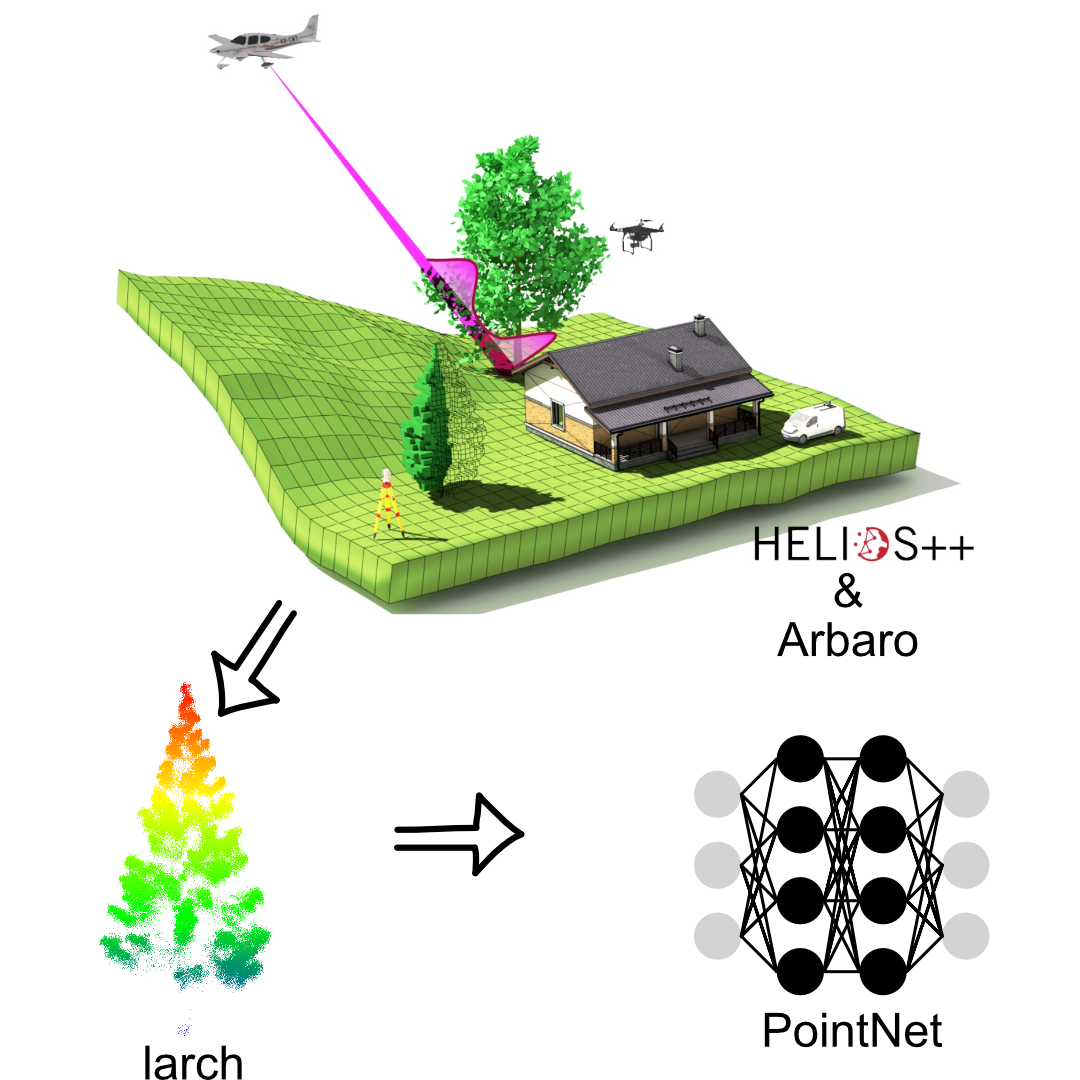
\includegraphics[width=0.5\textwidth]{assets/workflow_synthetic_data}
\caption[Workflow for generating synthetic lidar data ]{The workflow for generating synthetic lidar data starts with generating tree models. This is done with the software Arbaro\footnote{\url{https://github.com/wdiestel/arbaro}, accessed on: 22.02.2023}~(\cite{weber_1995_arbaro}). Based on these models, Helios++~(\cite{9906068}) is used to simulate lidar data which is similar to data capture with the Zenmuse L1 sensor from DJI\footnote{\url{https://www.dji.com/de/zenmuse-l1}, accessed on: 22.02.2023}. This generated data is used to pre-train a PointNet model proposed by ~\textcite{2017_qi_pointnet}. The figure is adapted from \textcite{9906068}.}
\label{fig:lidar-workflow}
\end{figure}

\subsection{Fundamentals of software profiling}
\label{sec:profiling}

% general introduction
Software profiling is "a form of dynamic program analysis (as opposed to static code analysis), is the investigation of a program's behavior using information gathered as the program executes"~(\cite{wiki:profiling}).
Metrics commonly of interest to identify performance bottlenecks are the number and elapsed time per function call and the memory consumption.

% definition of metrics
Metrics traditionally used for software profiling are execution time and \acf{FLOPS}~(\Cref{tab:metrics}).
Execution time is a simple measure that reports a function call's total time.
\ac{FLOPS} refers to the number of floating point operations that can be executed per second and can be used to evaluate the model's efficiency.

With the advent of \ac{GPU}'s throughput and \acf{MACs} gained importance~(\cite{verma_2019_metrics-ml-benchmarking}).
Throughput is essential as deep learning models need to analyze massive amounts of data to find generalizable patterns and can report on the model's speed.
Analog to \ac{FLOPS} \ac{MACs} do report on the software's efficiency. "Most modern hardware architectures use FMA [fused multiply-add] instructions for operations with tensors. FMA computes $a*x+b$ as one operation. Roughly $GMACs = 0.5 * GFLOPs$"\footnote{\url{https://github.com/sovrasov/flops-counter.pytorch/issues/16\#issuecomment-518585837} , accessed on: 22.11.2022}.

Further, profiling memory consumption is critical, as deep learning applications depend on massive amounts of data. Therefore, efficiently using \ac{GPU}'s internal memory is critical to the overall performance.

Other important profiling measures in deep learning, which are not considered in this report, are Time to Accuracy (TTA) and Average Time to Multiple Thresholds (ATTMT)~(\cite{verma_2019_metrics-ml-benchmarking}). These metrics were out of scope as the tested tools (\Cref{sec:tools-overview}) do not provide this information. However, setting up a workflow to measure these metrics based on the tools tested here is possible.

% Please add the following required packages to your document preamble:
% \usepackage{booktabs}
% \usepackage{multirow}
\begin{table}[H]
\centering
\begin{tabular}{@{}ll@{}}
\toprule
metric                                                                                 & purpose                        \\ \midrule
Execution time                                                                         & \multirow{2}{*}{traditionally} \\
FLOPS                                                                                  &                                \\ \midrule
Throughput: $\frac{images}{sec}$                                                       & \multirow{2}{*}{with the advent of GPUs} \\
MACs                                                                                   &                                \\ \bottomrule
\end{tabular}
\caption[Overview of performance metrics]{Overview of performance metrics that were used for profiling.}
\label{tab:metrics}
\end{table}

\subsection{Profiling tools}

\subsubsection{Overview of profiling tools}
\label{sec:tools-overview}

Many different profiling tools can be used to gain insights into the PyTorch workflow presented in~\Cref{sec:workflow} exist. 
~\Cref{tab:tools} lists some of the considered options.
General profiling tools such as Intel's Vtune~\footnote{\url{https://www.intel.com/content/www/us/en/developer/tools/oneapi/vtune-profiler.html}, accessed on: 22.11.2022} or the open-source software LIKWID\footnote{\url{https://github.com/RRZE-HPC/likwid}, accessed on: 22.11.2022} can be used to collect valuable metrics of any software.

However, tools were developed specifically to the needs one needs to profile PyTorch workflows.
One popular tool is the in-build PyTorch profiler, which can be combined with Tensorboard~\footnote{\url{https://www.tensorflow.org/tensorboard/}, accessed on: 16.03.2023}. This graphical visualization can be used for beginners and experts to optimize their workflows, as it provides automatic performance recommendations and detailed views such as the call stack or the trace view.
Another tool specifically designed for PyTorch is DeepSpeed~\footnote{\url{https://www.deepspeed.ai/tutorials/flops-profiler/}, accessed on: 16.03.2023}. The FlopsProfiler was used here, as the Pytorch Profiler lacks the option to analyze FLOPS.


General profiling tools could not provide automatic recommendations or useful visualizations to highlight critical aspects and bottlenecks, as they do not have insights into PyTorch. Consequently, more expert knowledge is required to use tools like LIKWID or Vtune.
As this project's research goal was identifying easy-to-use tools, this report focuses on the PyTorch Profiler and DeepSpeed's FlopsProfiler.

% Please add the following required packages to your document preamble:
% \usepackage{booktabs}
% \usepackage{multirow}
\begin{table}[H]
\centering
\begin{tabular}{@{}lll@{}}
\toprule
tool                              & metrics                                                                                & scope                    \\ \midrule
\href{https://pytorch.org/tutorials/intermediate/tensorboard_profiler_tutorial.html}{PyTorch Profiler With TensorBoard} & \begin{tabular}[c]{@{}l@{}}performance metrics\\ (e.g. time, memory)\end{tabular}      & \multirow{2}{*}{PyTorch} \\
\href{https://www.deepspeed.ai/tutorials/flops-profiler/}{Deepspeed/FlopsProfiler}                      & FLOPS                                                                                  &                          \\ \midrule
\href{https://www.intel.com/content/www/us/en/developer/tools/oneapi/vtune-profiler.html}{Vtune}                             & \multirow{2}{*}{\begin{tabular}[c]{@{}l@{}}general\\ performance metrics\end{tabular}} & Intel-only               \\
\href{https://github.com/RRZE-HPC/likwid}{likwid}                            &                                                                                        & general                  \\ \bottomrule
\end{tabular}
\caption[Overview of profiling tools]{Ovierview of tools used for profiling.}
\label{tab:tools}
\end{table}


\subsubsection{TensorBoard}
\label{sec:Tensorboard}

Tensorboard is "TensorFlow's visualization toolkit"~\footnote{\url{https://www.tensorflow.org/tensorboard}, accessed on: 20.3.2023} and is commonly used to visualize the loss and accuracy during the training process of a neural network.
For most people starting with deep learning, Tensorboard is one of the first tools to get insights into the deep learning workflow.
Unlike the name implies, this tool is not limited to using TensorFlow but can also be used with PyTorch.

\subsubsection{PyTorch - Profiler}
\label{sec:m-pytorch-profiler}

A more advanced option to get insights into a PyTorch Workflow is the PyTorch - Profiler, which is "a simple profiler API that is useful when user needs to determine the most expensive operators in the model"~\footnote{\url{https://pytorch.org/tutorials/recipes/recipes/profiler_recipe.html}, accessed on: 20.3.2023}.
With the help of this tool, one can collect general performance metrics, identify expensive operators, and track kernel activity.
The PyTorch - Profiler can be used with Tensorboard to visualize the profiling outputs~\footnote{\url{https://pytorch.org/tutorials/intermediate/tensorboard_profiler_tutorial.html}, accessed on: 20.3.2023}.


\subsubsection{Deepspeed - FlopsProfiler}
\label{sec:m-FLOPSprofiler}

DeepSpeed is a collection of tools that can help to optimize deep learning workflows~\footnote{\url{https://www.deepspeed.ai/}, accessed on: 20.3.2023}.
This project's primary interest was on the FlopsProfiler~\footnote{\url{https://www.deepspeed.ai/tutorials/flops-profiler/}, accessed on: 20.3.2023}. 
As the name implies, the FlopsProfiler can measure the efficiency (\ac{FLOPS}) for both the training and inference of a deep learning model. Further, it can profile the model's speed (latency, throughput).
Contrary to the PyTorch Profiler, the output is text-based without a visualization tool.


\subsection{Experiments}
\label{sec:m-experiments}

For the design of the experiments, two main questions were considered.
What is the benefit of using different accelerators? What is the cost/overhead of using profilers?

Therefore, the three presented tools~(\Cref{sec:tools-overview}) were tested on all available \ac{GPU}s of the \ac{SCC}\footnote{\url{https://www.gwdg.de/web/guest/hpc-on-campus/scc}}.
The main focus is on comparing the PyTorch - Profiler and DeepSpeed's Flops Profiler, as these tools are promoted primarily to optimize the performance of deep learning workflows. In addition, Tensorboard was included to analyze the overhead of this relatively simple and commonly used tool and to have a baseline for simple profiling tools.

\begin{figure}[H]
\centering
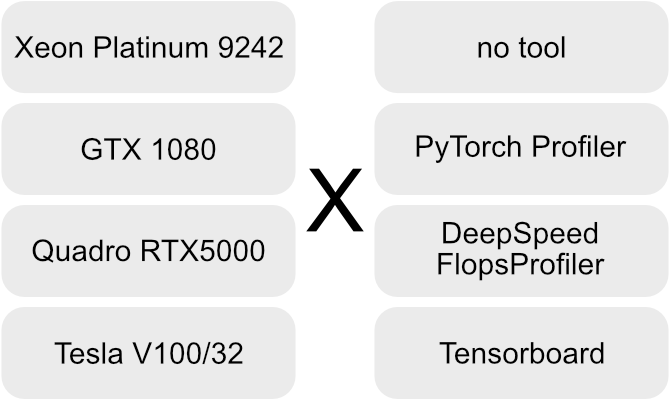
\includegraphics[width=0.5\textwidth]{./assets/experiments.png}
\caption[Overview of the runs]{In total, 16 different runs were planned by testing all possible combinations of tools with available \ac{GPU}s and one \ac{CPU}. Four more runs were performed by adding experiments according to the data loader process and different batch sizes (\Cref{tab:experiments-all}).}
\label{fig:experiments}
\end{figure}

Based on this experiment design, 16 different runs were executed~(\Cref{tab:experiments-all}).
Two more runs were included to test the performance recommendations of the PyTorch Profiler (runs 17 and 20).
Another two runs show the effect of an unoptimized data loading process, where the raw point cloud is loaded every time, and the point sampling process happens afterward (runs 18 and 19).

\begin{table}[H]
\centering
\begin{tabular}{@{}llllll@{}}
\toprule
run & node         & tool           & job\_id  & is\_valid & experiment     \\ \midrule
1   & scc\_cpu     & no-tool        & 14629421 & TRUE      &                \\
2   & scc\_cpu     & tensorboard    & 14629426 & TRUE      &                \\
3   & scc\_cpu     & profiler-torch & 14650740 & TRUE      &                \\
4   & scc\_cpu     & deepspeed      & 14617521 & FALSE     &                \\
5   & scc\_gtx1080 & no-tool        & 14619617 & TRUE      &                \\
6   & scc\_gtx1080 & tensorboard    & 14615343 & TRUE      &                \\
7   & scc\_gtx1080 & profiler-torch & 14650076 & TRUE      &                \\
8   & scc\_gtx1080 & deepspeed      & 14615344 & TRUE      &                \\
9   & scc\_rtx5000 & no-tool        & 14619618 & TRUE      &                \\
10  & scc\_rtx5000 & tensorboard    & 14617172 & TRUE      &                \\
11  & scc\_rtx5000 & profiler-torch & 14650079 & TRUE      &                \\
12  & scc\_rtx5000 & deepspeed      & 14617171 & TRUE      &                \\
13  & scc\_v100    & no-tool        & 14619619 & TRUE      &                \\
14  & scc\_v100    & tensorboard    & 14617203 & TRUE      &                \\
15  & scc\_v100    & profiler-torch & 14650080 & TRUE      &                \\
16  & scc\_v100    & deepspeed      & 14617202 & TRUE      &                \\
17  & scc\_gtx1080 & profiler-torch & 14650758 & TRUE      & batch-size-64  \\
18  & scc\_gtx1080 & profiler-torch & 14650750 & TRUE      & sample-points  \\
19  & scc\_cpu     & profiler-torch & 14657599 & TRUE      & sample-points  \\
20  & scc\_gtx1080 & profiler-torch & 14650759 & TRUE      & batch-size-128 \\ \bottomrule
\end{tabular}
\caption[Overview of all runs]{In total, twenty different experiments were performed. The first 16 experiments are directly derived from the experiment design presented in \Cref{fig:experiments}. Experiments 18 and 19 were preliminary work to optimize the data loading process before all experiments were performed (~\Cref{sec:r-data-loading}). Experiments 17 and 20 were done based on the PyTorch - Profiler's performance recommendations(~\Cref{sec:r-pytorch-profiler}).}
\label{tab:experiments-all}
\end{table}

\section{Results}
\label{sec:results}

\subsection{Optimization of the data loading process}
\label{sec:r-data-loading}

As we were aware that due to the massive amount of data we want to process, the data loading process is a bottleneck, it was decided to optimize this aspect before doing all remainig runs presented in~\Cref{sec:m-experiments}. This way, it was possible to run more experiments without wasting valuable \ac{GPU} hours for all users on the \ac{SCC}. The idea is to speed up the data-loading process by migrating the point sampling to a pre-processing workflow. Point sampling means selecting the number of points per tree the neural network architecture pointnet expects as input. Thus, it is possible to reduce the data size by a factor of $ 1714.55 $, from $931 GB $ to $543 MB $. 

As the data loading process was the major bottleneck, reducing data that needs to be loaded during the training process significantly speeds up the whole training workflow. For example, while it still took $~4 hours$ to train the network on the GTX 1080 in the unoptimized version, it only took $~16 minutes$ for the optimized version. Similarly, the training process on the \ac{CPU} was decreased from $~14$ hours and $15$ minutes to $~2$ hours and $49$ minutes. This means a speed up for the \ac{CPU} by a factor of $~5$ and for the \ac{GPU} (GTX 1080) a speed up by a factor of $~14$.

So far, the optimization problem has been solved by expert knowledge about the workflow and the data. Simultaneously the PyTorch - Profiler was tested to identify the bottleneck in the data loader. Unfortunately, the overview did not help identify the issue. Only an analysis of the trace view revealed that the function for reading the data takes up a large part of the time and thus slows down the workflow (\Cref{fig:scap_gtx1080_profiler-torch_batch-size-64_14650758_trace-view-laspy}). More details on the PyTorch - Profiler can be found in~\Cref{sec:r-pytorch-profiler}.

\begin{figure}[H]
\centering
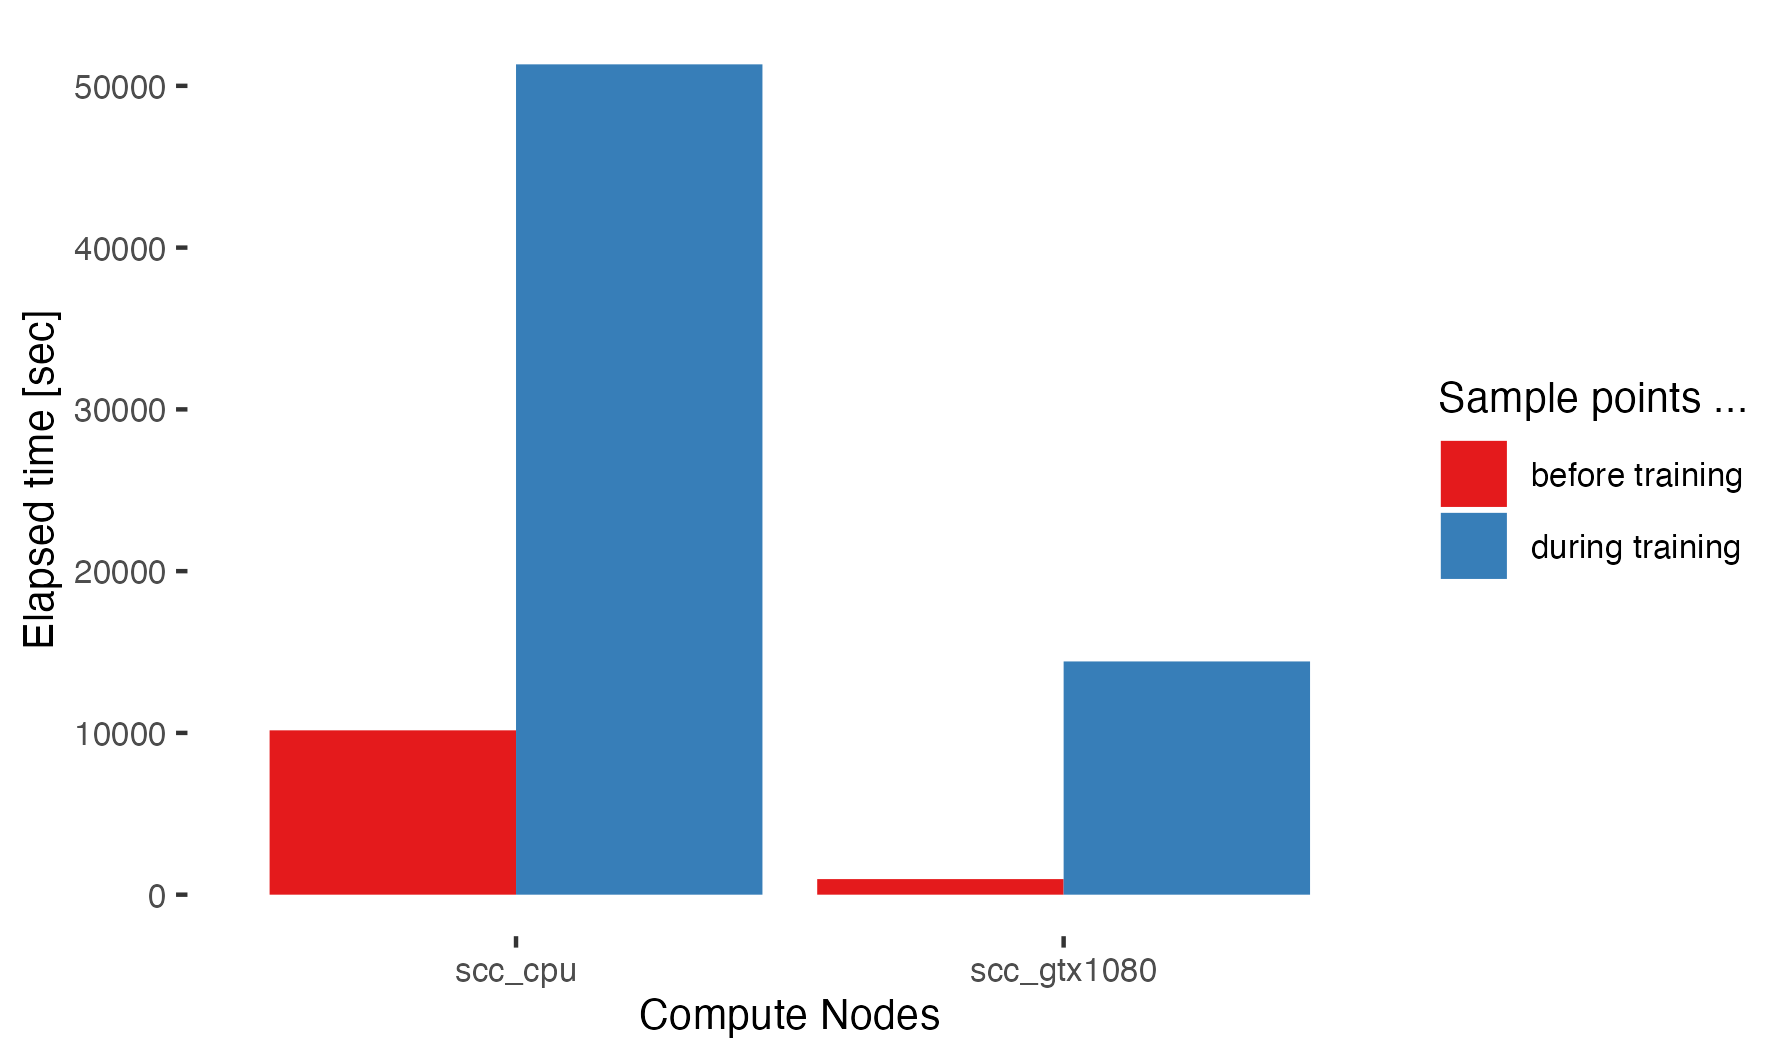
\includegraphics[width=1\textwidth]{./assets/sacct_barplot_by_nodes_sample-points-effect}
\vspace{-1em}
\caption[Effect of the data loading optimization]{By migrating the point sampling process from the data loader to a pre-processing step, the elapsed time for the training runs was decreased significantly.}
\label{fig:sacct_barplot_by_nodes_sample-points-effect}
\end{figure}

\subsection{Effect of the accelerators and profiling tools on the runtime}
\label{sec:r-runtime}

The simplest method to get a first estimate for the performance of all different runs is to look at the elapsed time for each analysis. On the \ac{SCC} jobs are executed via SLURM~\footnote{\url{https://slurm.schedmd.com/}, accessed on: 21.3.2023} which provides the tool \texttt{sacct}\footnote{\url{https://slurm.schedmd.com/sacct.html}, accessed on: 21.3.2023} for analyzing accounting information, such as elapsed time of a job. The raw output and the command to get this information can be found in the Appendix (~\Cref{lst:sacct_out}, \Cref{lst:sacct_command}). 

Most apparent is the difference between runs on the \ac{CPU} and the \ac{GPU}s (\Cref{fig:sacct_barplot_by_nodes_no-experiment}). The mean runtime for jobs on \ac{CPU}s is $9669.333$ seconds, and for runs on the \ac{GPU}s, $513.25$ seconds. Further, it is notable that DeepSpeed is not compatible with \ac{CPU}s. A more detailed view on runs using the \ac{GPU}s (\Cref{fig:sacct_barplot_by_nodes_no-experiment_gpu}) shows that the GTX 1080 node is slower (mean runtime of $13$ minutes) than the RTX 5000 node (mean runtime of $7.65$ minutes). The fastest node is the V100, with a mean runtime of $5.02$ minutes.

No clear trend can be observed regarding the overhead of the different profiling tools. Generally, the PyTorch - Profiler creates the highest overhead. However, on nodes GTX 1080 and RTX 5000, runs using DeepSpeed's FlopsProfiler or TensorBoard are faster than baseline runs without any tools.

\begin{figure}[H]
\centering
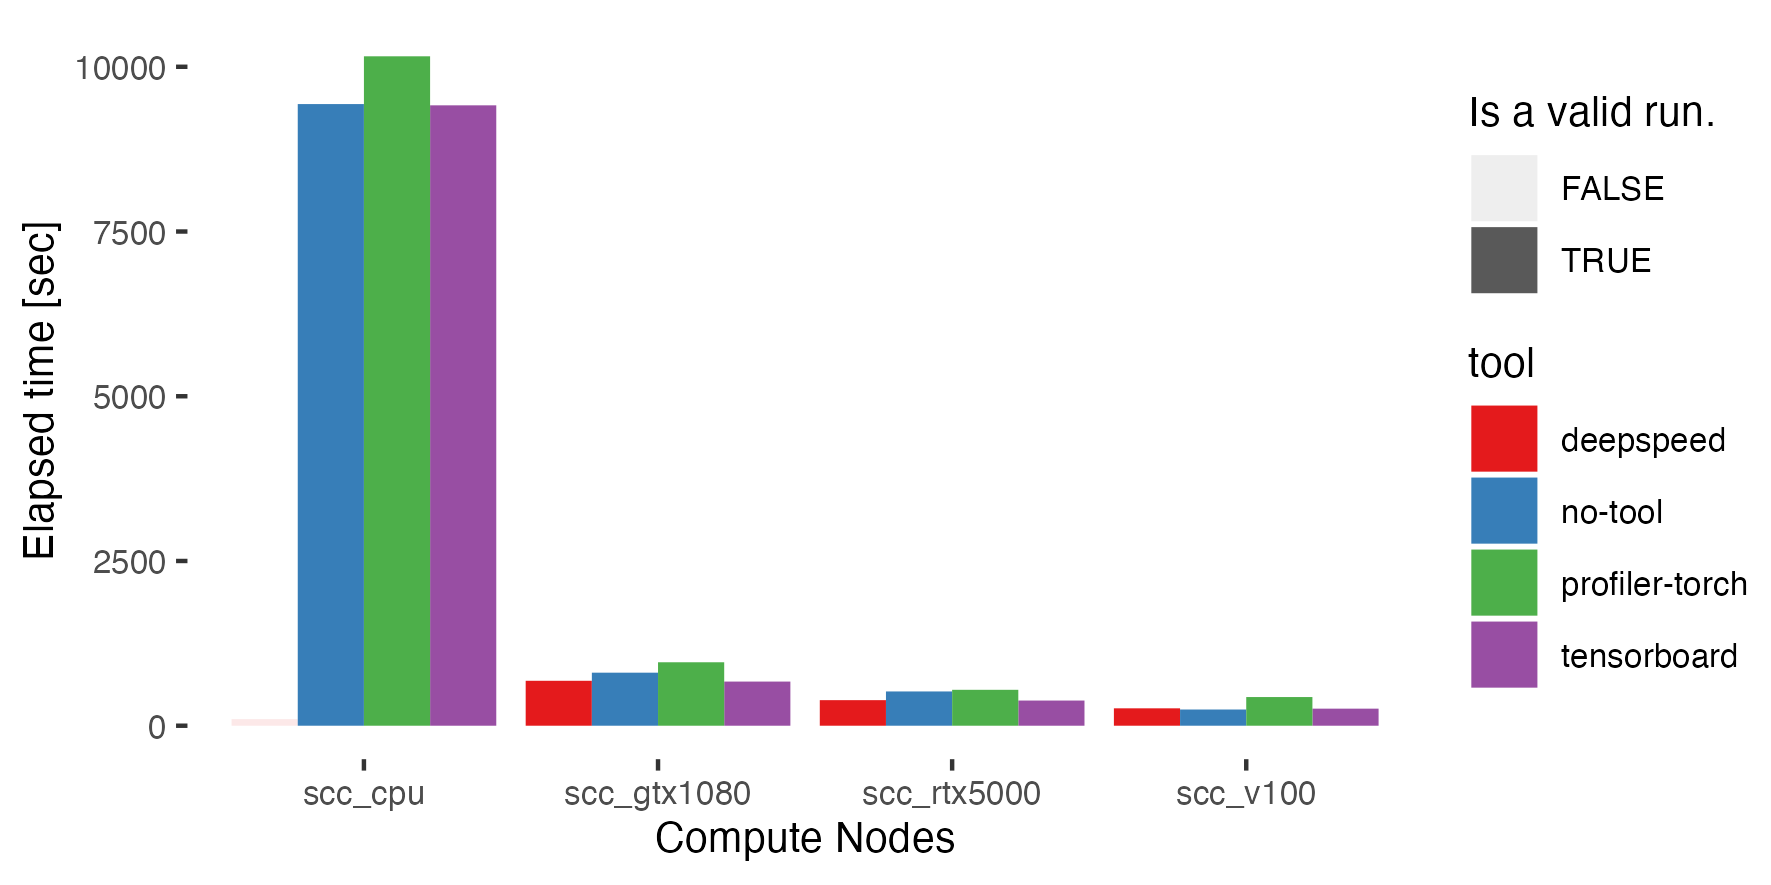
\includegraphics[width=1\textwidth]{./assets/sacct_barplot_by_nodes_no-experiment}
\caption[Runtime of the experiments]{The runtime of all runs testing the combination of tools and \ac{GPU} and \ac{CPU} partitions (\Cref{fig:experiments}). }
\label{fig:sacct_barplot_by_nodes_no-experiment}
\end{figure}

\begin{figure}[H]
\centering
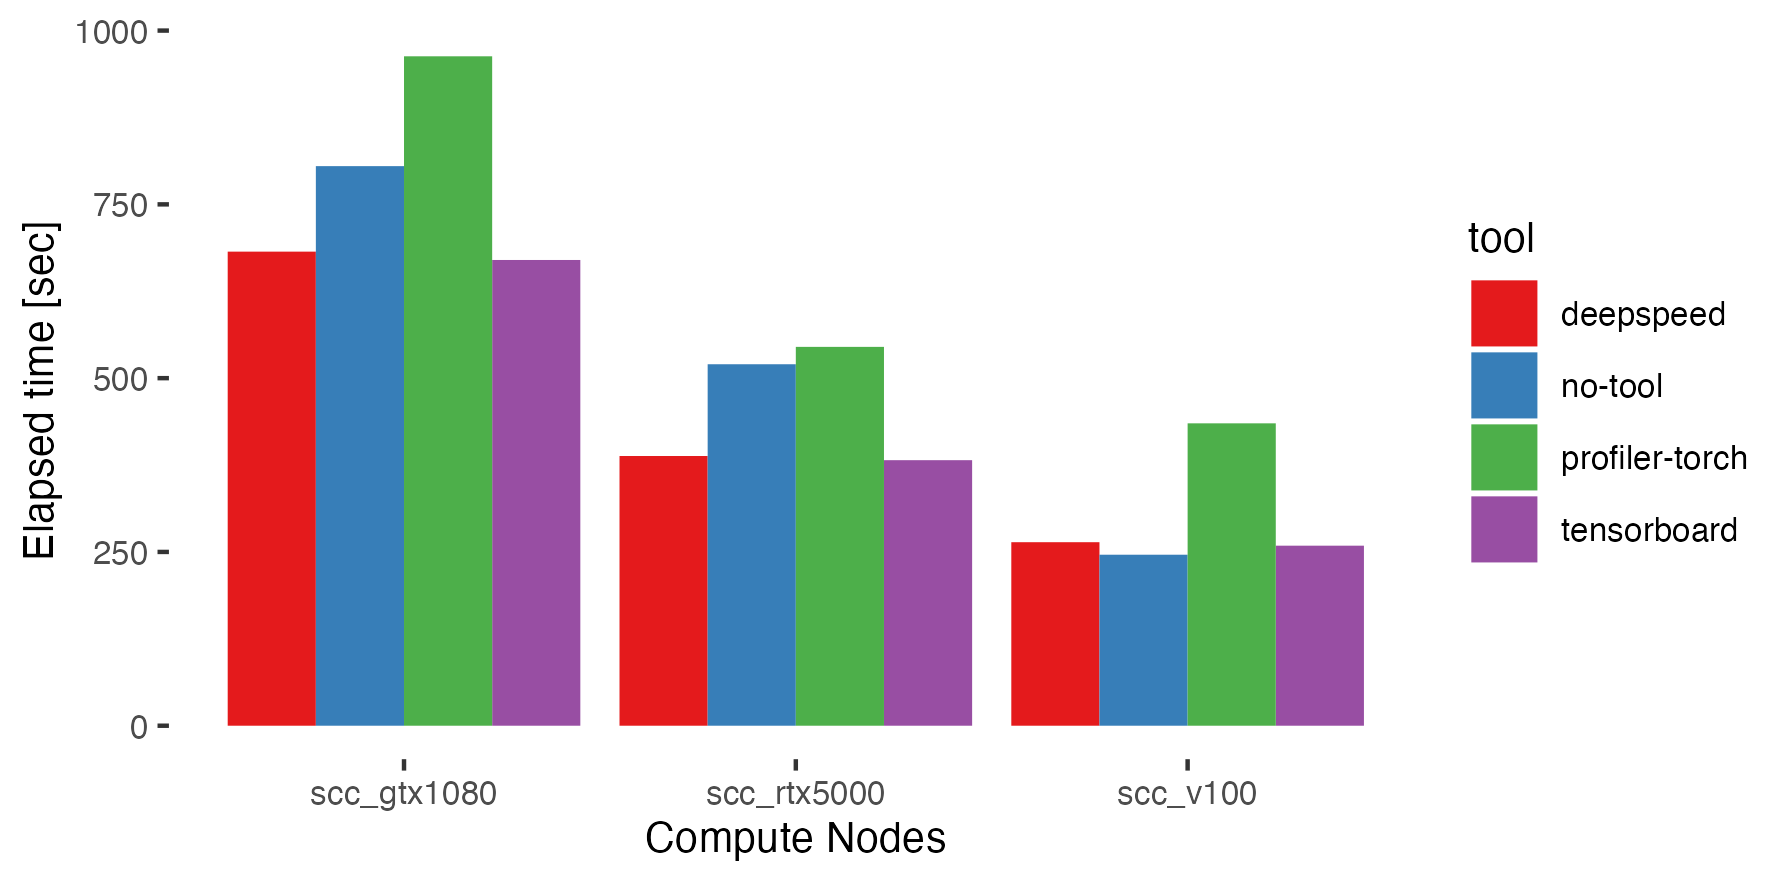
\includegraphics[width=1\textwidth]{./assets/sacct_barplot_by_nodes_no-experiment_gpu}
\caption[Runtime of the experiments (GPU-only)]{The runtime of all runs testing the combination of tools and \ac{GPU} partitions - excluding \ac{CPU} partitions (\Cref{fig:experiments}).}
\label{fig:sacct_barplot_by_nodes_no-experiment_gpu}
\end{figure}

\subsection{Results of the profiling tools}

\subsubsection{TensorBoard}
\label{sec:r-tensorboard}

The minimal example for using a TensorBoard to keep track of the model's training process provides information about the model's accuracy, the loss per epoch, and the loss per minibatch~(\Cref{fig:scap_gtx1080_tensorboard_14615343}). It can be seen that over the training time, the accuracy constantly increases, and the loss decreases.

\subsubsection{PyTorch - Profiler}
\label{sec:r-pytorch-profiler}

When visualizing the profiling results of the PyTorch Profiler with Tensorboard, the first view visible is the "Overview". This view is one of six different views, showing different details of the profiler output. If not labeled differently here, the output of the PyTorch - Profiler run on the GTX 1080 with optimized batch size of 64~(run 17 \Cref{tab:experiments-all}) will be discussed.

The "Overview"~(\Cref{fig:scap_gtx1080_profiler-torch_14650076}) gives "a high-level summary of the model performance"~\footnote{\url{https://pytorch.org/tutorials/intermediate/tensorboard_profiler_tutorial.html}, accessed on: 20.3.2023}. It can be subdivided into five different panes. On top, there are the panes "Configuration", "GPU Summary", and "Execution Summary". In "Configuration", information about the number(s) of workers and device type (\ac{CPU} or \ac{GPU}) are listed. The "GPU Summary" provides information about the GPU utilization by showing different metrices~\footnote{\url{https://pytorch.org/tutorials/intermediate/tensorboard_profiler_tutorial.html}, accessed on: 22.3.2023}, such as "GPU Utilization" and the "Estimated Stream Multiprocessor Efficiency". Here the metrics indicate that the utilization of the GPU is relatively low for the tested workflow. The same can be seen in the "Execution Summary", where the time spent on the kernel is low. Here, the profiler misses detecting the DataLoader operations and sums up most of the time spent for the workflow in the category "Other". The "Step Time Breakdown" visualizes the same information as the "Execution Summary" per step. However, in the tested example, just the first step was visualized. The last pane, "Performance Recommendation", provides hints for optimizing the PyTorch workflow. Here, the profiler detected a low \ac{GPU} utilization where a common strategy is to increase the batch size. Testing this recommendation showed that increasing the batch size from 32 to 64 improved the GPU utilization by $~10\%$~(\Cref{fig:scap_gtx1080_profiler-torch_comparison-batch-size}). As the utilization is still low, the performance recommendation remains the same. Nevertheless, increasing the batch size to 64 lead to a decrease in GPU utilization.

\begin{figure}[H]
\centering
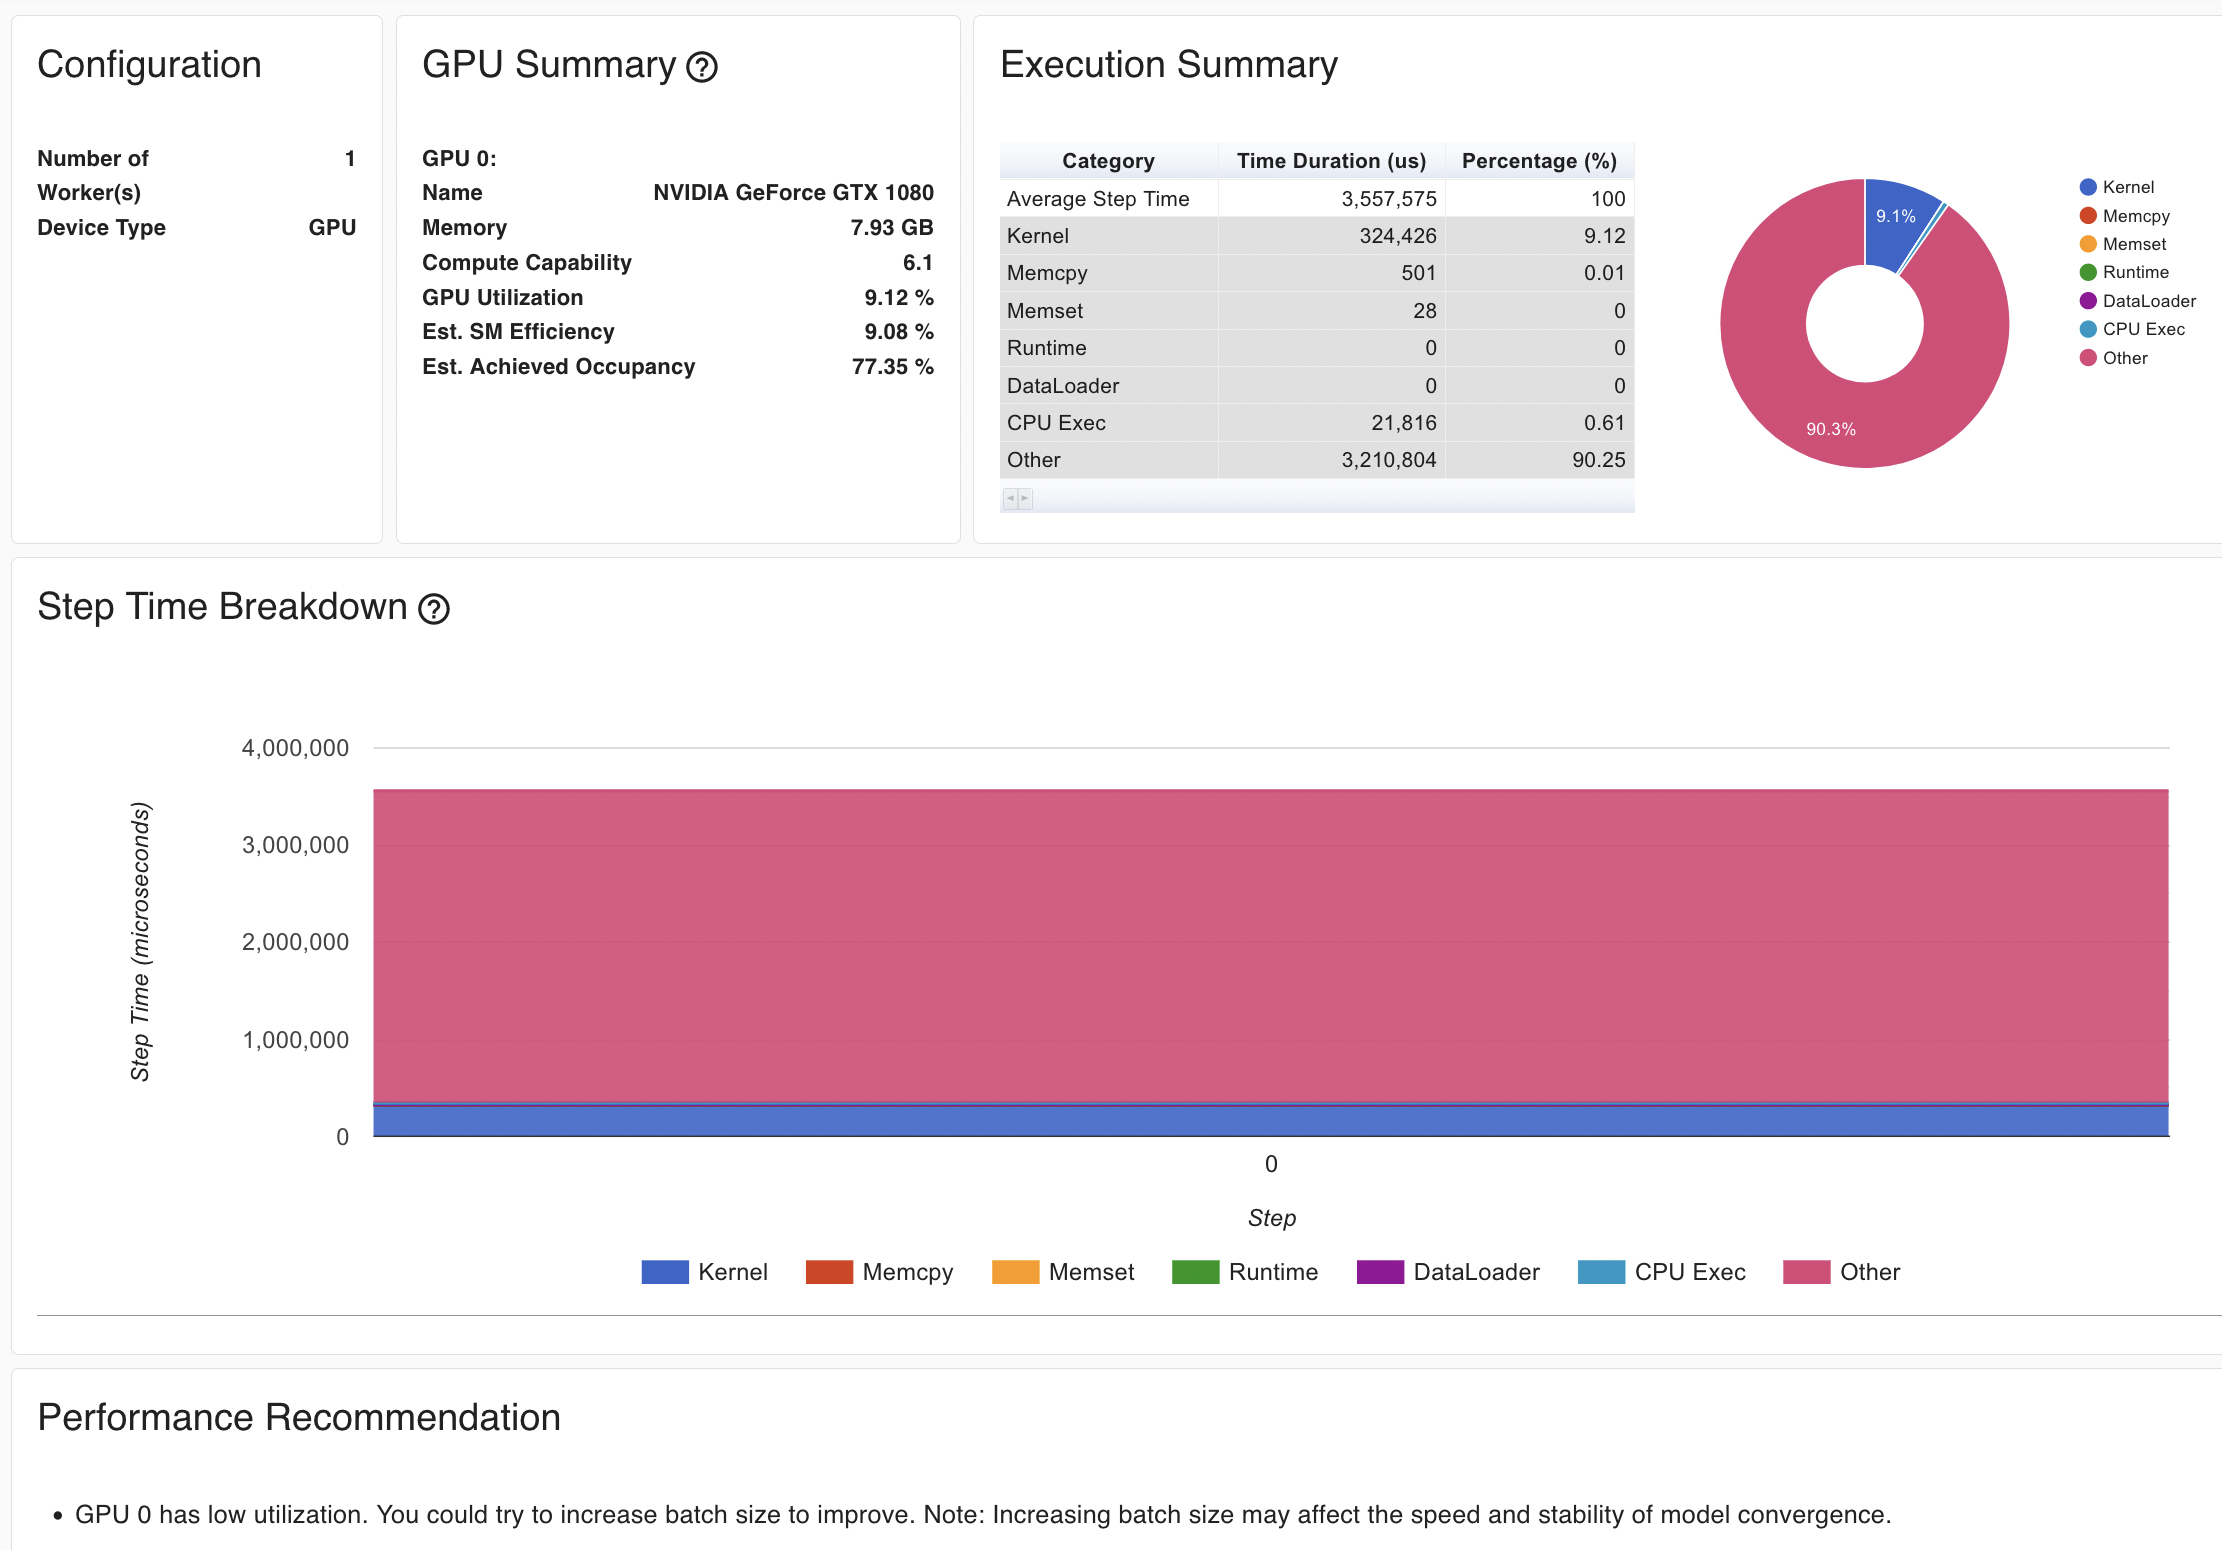
\includegraphics[width=0.95\textwidth]{./assets/scap_gtx1080_profiler-torch_14650076}
\vspace{-0.5em}
\caption[PyTorch - Profiler: Overview]{Visualizing the profiling results of the PyTorch - Profiler with Tensorboard provides an overview page. This page summarizes important metrics of the workflow, such as \ac{GPU} utilization. Details on the metrics can be found in the corresponding Github repository~\footnote{\url{https://github.com/pytorch/kineto/blob/main/tb_plugin/docs/gpu_utilization.md}, accessed on: 27.22023}. Further, it offers performance recommendations on how to adress potential bottlenecks. This "Overview" shows the result for run 17 in \Cref{tab:experiments-all}.}
\label{fig:scap_gtx1080_profiler-torch_14650076}
\end{figure}

\begin{figure}[H]
\centering
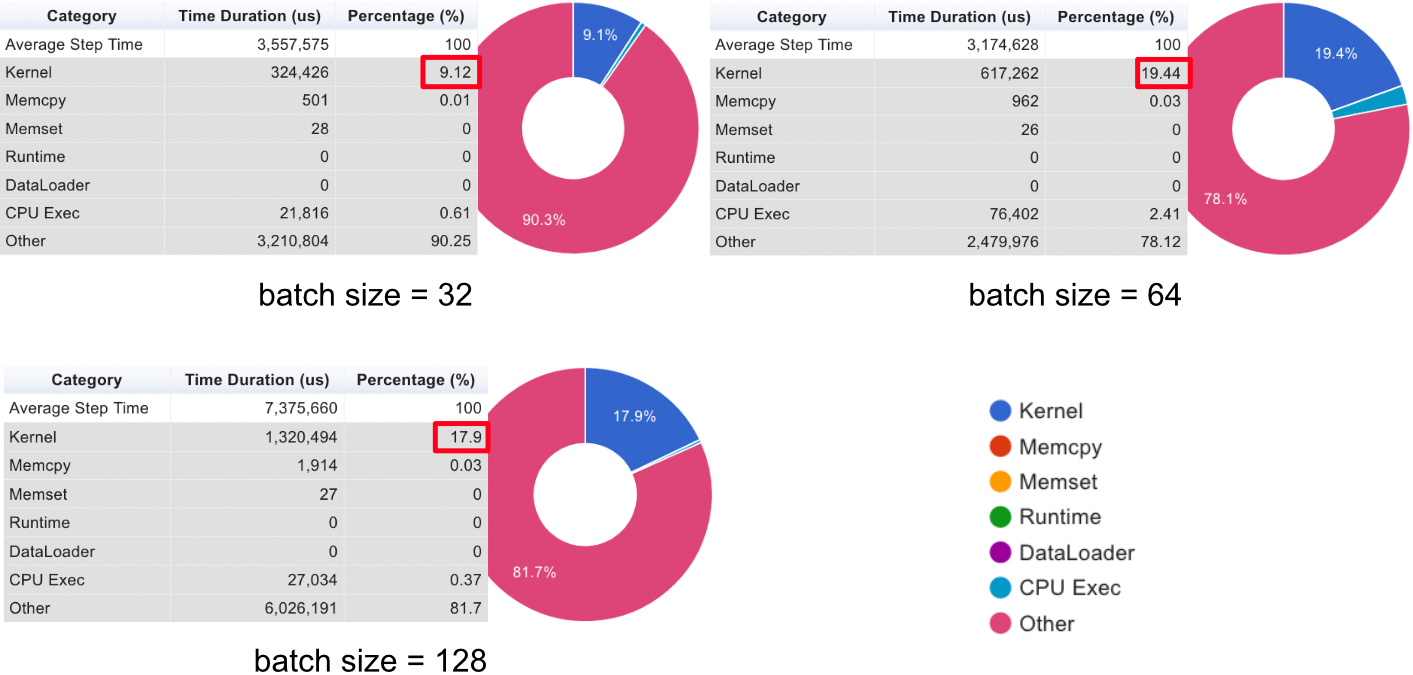
\includegraphics[width=0.95\textwidth]{./assets/scap_gtx1080_profiler-torch_comparison-batch-size}
\vspace{-0.5em}
\caption[PyTorch - Profiler: Performance Recommendation]{For the tested training workflow the performance recommendations of the PyTorch - Profiler suggest to increase the batch size. The effect of the batch size on the \ac{GPU} utilization can be seen for a batch size of 32 (run 7 in~\Cref{tab:experiments-all}), 64 (run 17 in~\Cref{tab:experiments-all}), 128 (run 20 in~\Cref{tab:experiments-all}). The full view for these experiments can be seen in~\Cref{fig:scap_gtx1080_profiler-torch_14650076}, \Cref{fig:scap_gtx1080_profiler-torch_batch-size-64_14650758}, and \Cref{fig:scap_gtx1080_profiler-torch_batch-size-128_14650759}.}
\label{fig:scap_gtx1080_profiler-torch_comparison-batch-size}
\end{figure}

The "Trace View" of the PyTorch - Profiler shows the usage of operators and GPU kernels on a timeline~(\Cref{fig:scap_gtx1080_profiler-torch_batch-size-64_14650758_trace-view}). By clicking on operators, details, such as start time or end time, can be seen (\Cref{fig:scap_gtx1080_profiler-torch_batch-size-64_14650758_trace-view-laspy}). Further, this view provides insights into operator connections ("incoming flow").
As already stated in the "Overview", it can be seen that the GPU is most of the time waiting for other operators on the CPU to finish. That way, a significant part of the GPU time is wasted. The operator identified as a bottleneck is the data reading operation. This is even worse for the not optimized workflow (run 18~\Cref{tab:experiments-all}) where the raw point cloud is loaded and afterward, the point sampling is done (\Cref{fig:scap_gtx1080_profiler-torch_sample-points_14650750_trace-view-laspy}). For one reading operation, the optimized data loading strategy takes $3,023$ milliseconds, and the unoptimized variation requires $58,064$ milliseconds.

\begin{figure}[H]
\centering
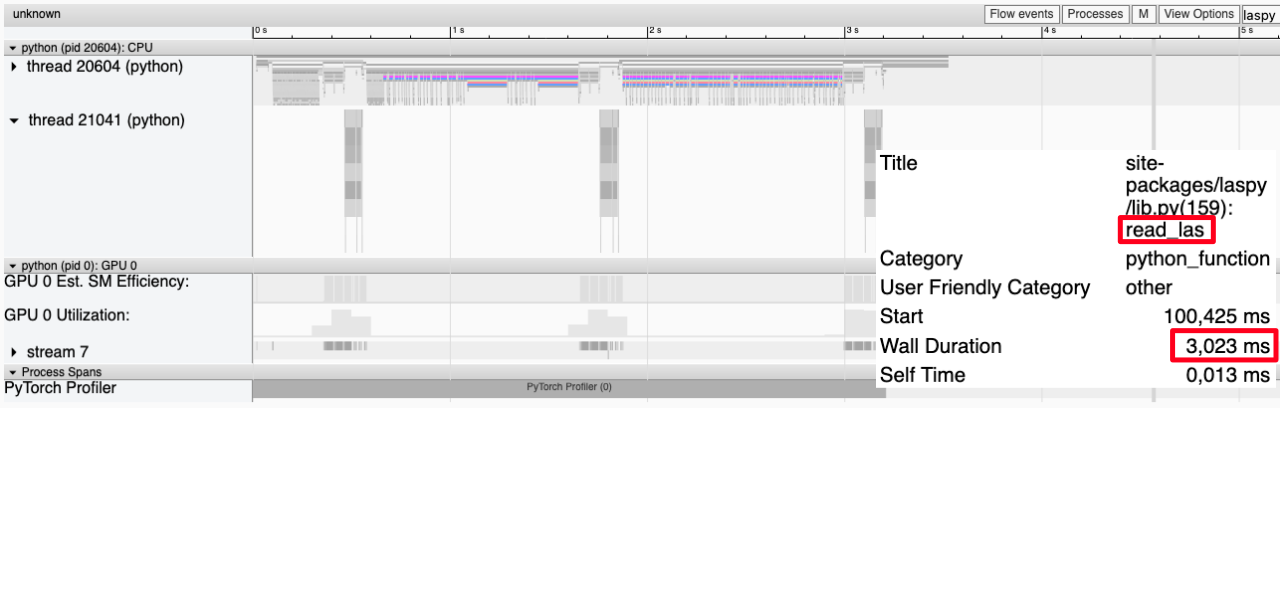
\includegraphics[width=1\textwidth]{./assets/scap_gtx1080_profiler-torch_batch-size-64_14650758_trace-view-laspy}
\vspace{-6em}
\caption[PyTorch - Profiler: Trace View of data input]{The "Trace View" provides insights into the operators and GPU kernels over time. Here the read operation of the lidar data based on pre-sampled point clouds is analyzed.}
\label{fig:scap_gtx1080_profiler-torch_batch-size-64_14650758_trace-view-laspy}
\end{figure}

\begin{figure}[H]
\centering
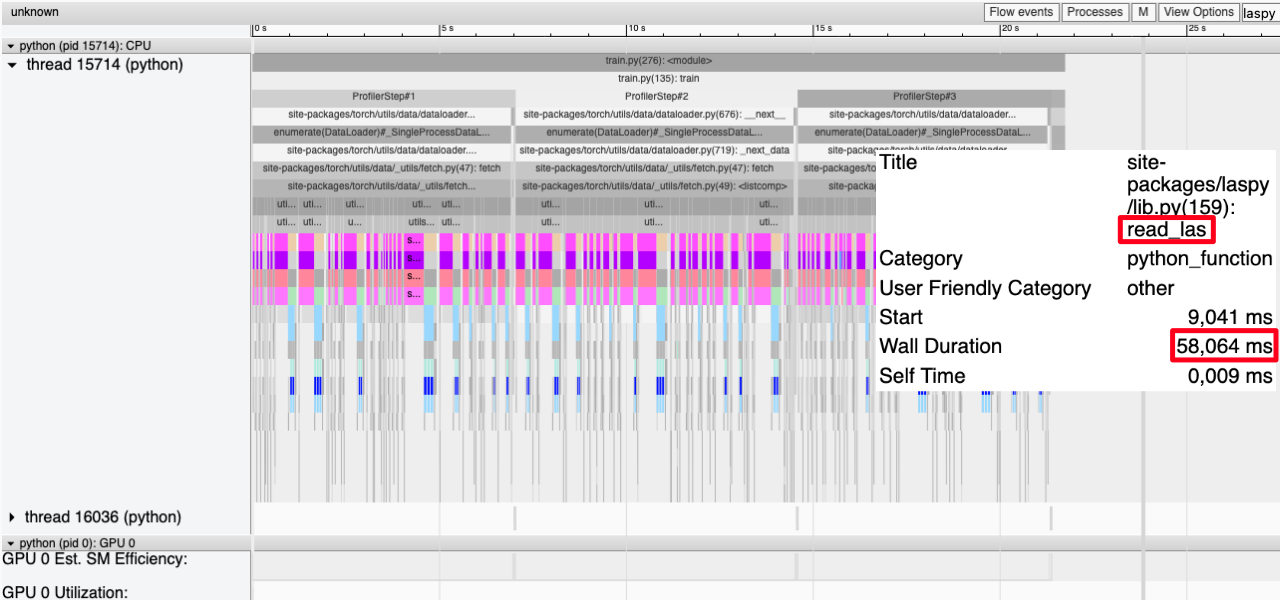
\includegraphics[width=1\textwidth]{./assets/scap_gtx1080_profiler-torch_sample-points_14650750_trace-view-laspy}
\caption[PyTorch - Profiler: Trace View of data input for run 18]{The trace view of the unoptimized workflow (run 18~\Cref{tab:experiments-all}), loading the raw lidar data, shows that a significant part of the time is spend on the reading opertions.}
\label{fig:scap_gtx1080_profiler-torch_sample-points_14650750_trace-view-laspy}
\end{figure}

Different views provided by the PyTorch - Profiler are "Operator", "GPU Kernel", "Memory", and "Module".
The "Operator" view provides insights into the profiling results of PyTorch's operators~(\Cref{fig:scap_gtx1080_profiler-torch_batch-size-64_14650758_operator-view}). Self-time refers to the duration of the operator without child operators, which are included in the total time. For example, it can be seen that the operator \texttt{aten::copy\_} is expensive. Also, the View CallStack can be shown in this view~(\Cref{fig:scap_gtx1080_profiler-torch_batch-size-64_14650758_operator-view-details}).
The "GPU Kernel" view shows for all kernels the time that was spent on the \ac{GPU}~(\Cref{fig:scap_gtx1080_profiler-torch_batch-size-64_14650758_gpu-kernel-view}). More information about the metrics used in this view can be found on the official tutorials website\footnote{\url{https://pytorch.org/tutorials/intermediate/tensorboard_profiler_tutorial.html}, accessed on: 20.3.2023}.
The "Memory" view gives information about memory usages, such as allocation and release events. This view consists of a "memory curve graph, memory events table, and memory statistics table"\footnote{\url{https://pytorch.org/tutorials/intermediate/tensorboard_profiler_tutorial.html}, accessed on: 20.3.2023}~(\Cref{fig:scap_gtx1080_profiler-torch_batch-size-64_14650758_memory-view}).
The "Module" view shows profiling results (occurrences, time) per PyTorch module, such as the whole PointNet or the submodule Transform~(\Cref{fig:scap_gtx1080_profiler-torch_batch-size-64_14650758_module-view}).


\subsubsection{DeepSpeed - FlopsProfiler}
\label{sec:r-flopsprofiler}

The output of the DeepSpeed - Flops Profiler is a textfile~(\Cref{lst:scap_gtx1080_deepspeed_14615344_4294967294_one-epoch-full}), which provides metrics on different levels of the network. The first part summarizes metrics for the whole neural network, such as the model parameters, \ac{MACs}, number of floating-point operations (flops), floating-point operations per second (FLOPS), and latency. Precise definitions of these metrics can be found in the output file~(\Cref{lst:scap_gtx1080_deepspeed_14615344_4294967294_one-epoch-full}). For this example run~(run 8 \Cref{tab:experiments-all}), a total of $14.07$ GMACs ($29.04$ Gflops) were measured. Dividing this by the forward propagation latency shows that for the whole model, the floating-point operations per second are $349.1$ GFLOPS.

\begin{listing}[H]
\inputminted[xleftmargin=1em,linenos,fontsize=\small, firstline=2,lastline=16, breaklines]{python}{./assets/scap_gtx1080_deepspeed_14615344_4294967294_one-epoch.txt}
\caption{DeepSpeed - FlopProfiler: Summary}
\label{lst:scap_gtx1080_deepspeed_14615344_4294967294_one-epoch-summary}
\end{listing}

The second part of the DeepSpeed - FlopsProfiler's output~(\Cref{lst:scap_gtx1080_deepspeed_14615344_4294967294_one-epoch-aggregated}) reports on the top modules in different depths of the model. Top modules are defined based on the number of parameters, \ac{MACs}, and forward propagation latency are considered. In-depth 0 the whole PointNet model is considered so that the profiling results are the same as in the first part of the output~(\Cref{lst:scap_gtx1080_deepspeed_14615344_4294967294_one-epoch-summary}).
In depth 1 it can be seen that most of the resources are spent on the Transform module. For example, $14.05$ GMACs out of $14.07$ GMACs are spent on this module.
The top module in depth 2 is the Tnet with $9.34$ GMACs.

\begin{listing}[H]
\inputminted[xleftmargin=1em,linenos,fontsize=\small, firstline=19,lastline=31, breaklines]{python}{./assets/scap_gtx1080_deepspeed_14615344_4294967294_one-epoch.txt}
\caption{DeepSpeed - FlopProfiler: Aggregated Profile per GPU}
\label{lst:scap_gtx1080_deepspeed_14615344_4294967294_one-epoch-aggregated}
\end{listing}

In the detailed profile, the metrics are reported for all submodules of the model~(\Cref{lst:scap_gtx1080_deepspeed_14615344_4294967294_one-epoch-detailed}). Besides the metrics given for higher-level summarization before, e.g., metrics for the whole PointNet, all metrics for submodules are listed. The order of the metrics is params, percentage of total params, MACs, percentage of total MACs, fwd latency, percentage of total fwd latency, fwd FLOPS~(\Cref{lst:scap_gtx1080_deepspeed_14615344_4294967294_one-epoch-full}). For example, it can be seen that the second convolution of the Tnet is a 1D convolution\footnote{\url{https://pytorch.org/docs/stable/generated/torch.nn.Conv1d.html}, accessed on: 23.3.2023} with $268.44$ MMACs.

\begin{listing}[H]
\inputminted[xleftmargin=1em,linenos,fontsize=\small, firstline=41,lastline=48, breaklines]{python}{./assets/scap_gtx1080_deepspeed_14615344_4294967294_one-epoch.txt}
\caption{DeepSpeed - FlopProfiler: Detailed Profile per GPU}
\label{lst:scap_gtx1080_deepspeed_14615344_4294967294_one-epoch-detailed}
\end{listing}

\subsubsection{Usability of the different tools}
\label{sec:r-usability}

The tools provide different \ac{API}s, such as a context manager, as a decorater, or a Python module\footnote{\url{https://www.alcf.anl.gov/sites/default/files/2022-08/Profiling.pdf}, accessed on: 23.3.2023}. For example, the DeepSpeed Flops Profiler can be activated in DeepSpeed's runtime, which would not require to adapt the Python code at all. However, for this project all tools were used as Python packages. This requires to insert a few lines of code (8 to 13). The important parts of the code and their placement in the training code is shown in ~\Cref{lst:tensorboard}, \Cref{lst:profiler-torch}, and \Cref{lst:deepspeed}.
%todo how to parse the profiling output


\section{Discussion}
\label{sec:discussion}

Generally, the used profilers, PyTorch Profiler and DeepSpeed's FlopsProfiler, provide interesting and valuable insights into the training process of a PyTorch model, which can be used for optimization purposes. Nevertheless, also with the beginner-friendly TensorBoard approach, tracking the accuracy and loss, details of the training process can be analyzed.

The data loading process was the most apparent bottleneck for the PointNet workflow analyzed for this report. This bottleneck was seen in the PyTorch Profiler's logs and using expert knowledge about the size of the input data and the point data sampling technique within the data loader. 
In \Cref{fig:sacct_barplot_by_nodes_sample-points-effect}, two essential aspects for optimizing the PointNet workflow can be seen. First, the speedup for each compute node by migrating the point sampling process to a pre-processing step of the workflow. Second, there is a substantial difference between the runtimes of the \ac{CPU} and \ac{GPU}. Here it can be seen how important the use of accelerators, such as \ac{GPU}s, is for training deep neural networks.
Further, \Cref{fig:sacct_barplot_by_nodes_no-experiment_gpu} shows the performance gain one can get by using faster \ac{GPU} nodes on the cluster and the compute overhead each tool is generating due to its measurement activities and the writing of logging files. The overhead created by the PyTorch Profiler seems to be the highest. Interestingly, the runs without any tool on the GTX 1080 and RTX 5000 are slower than those profiled with DeepSpeed's FlopsProfiler and TensorBoard.
However, the mean of several identical runs would be required for a reliable performance comparison. Additionally, a performance comparison between nodes on the \ac{SCC} is more complicated because the compute nodes are shared resources, and computations by other users could affect the measurements. 

An easy starting point for profiling the training process of a PyTorch model is TensorBoard. Most will be familiar with this tool as it is commonly used in beginner introductions to deep learning. In addition, the user-friendly visualization as a dashboard and the interactivity increases the accessibility.
For example, the loss and accuracy curves shown in TensorBoard make overfitting visible, and the training process could be stopped manually or by early stopping rules. Additionally, checkpoints can prevent the re-training of models in such a case. These easy strategies for reducing the cost of training neural networks are also recommended by the authors of the paper Green AI~\cite{schwartz_2019_greenai} in their interview at the Practical AI podcast\footnote{\url{https://changelog.com/practicalai/124}, accessed on: 30.3.2023}.

Also, the PyTorch Profiler profits from intuitive visualizations in Tensorboard.
Especially the Overview page, with its performance recommendations, can be handy for beginners. Nevertheless, the effect of these recommendations should still be checked, as was shown in~\Cref{fig:scap_gtx1080_profiler-torch_comparison-batch-size}.
Further, the Trace view provided essential insights into the training workflow, highlighting the most resource intense operators. This helped identify the data reading as a bottleneck of the workflow.
More complicated is the evaluation of the other views, which report on the model's performance on a low level and sometimes require knowledge about the implementation of PyTorch and the model's architecture to make good use of it. 

As the PyTorch Profiler lacks the feature to measure \ac{FLOPS}, DeepSpeed's FlopsProfiler was additionally tested. The text-based logging file is easy to interpret for high-level summarizations of the model's performance~(\Cref{lst:scap_gtx1080_deepspeed_14615344_4294967294_one-epoch-full}). The "Detailed Profile per GPU" is less intuitive, which includes the measurements for all submodules in PyTorch. However, the "Aggregated Profile per GPU" already highlights the most expensive modules in different depths of the model. The analysis of the details view can then be limited to those modules.
Compared to example outputs in the official tutorial\footnote{\url{https://www.deepspeed.ai/tutorials/flops-profiler/}, accessed on: 24.3.2023}, some metrics are unfortunately not reported, such as the model's throughput. Further, there were issues about the compatibility with 3D convoultions\footnote{\url{https://github.com/microsoft/DeepSpeed/issues/1467}, accessed on: 24.3.2023}, which shows the importance of testing these tools with models one is interested in and not only the provided examples.

All tested tools were easy to use, and the effort to get them running was relatively low. However, they have some bugs or unexpected behaviors (just one step in the PyTorch Profiler, missing metrics in the FlopsProfiler), which could be reasoned by a wrong usage or actual bugs in the software. Unfortunately, figuring this out was out of the scope of this report.
\iffalse

optimize data loader
    - speed up bei GTX1080 deutlich höher (factor 5 gegen 14) -> bei der GPU deutlich größerer anteil an verlangsamenden komponenten. bei der CPU sind andere faktor auch massgeblich daran beteiligt
        -> darum accelerator für train of dl so wichtig

Effect of the accelerators and profiling tools on the runtime
- runtime shows which nodes are the fastest
    - CPUs are not optimized for this task
    - the faster the GPU the faster the training -> workflow can make use of faster hardware
    - overhead of PyTroch - Profiler is high
    - deepspeed/tensorboard runs faster than baseline run without tool
        - shared ressources
        - more reliable would be the mean of multiple runs and using one node exclusively
            - not done here as one run is sufficient to get an idea of the trend
            - do not waste energy/ressources
        - overhead seems to be nor too significant

tools

tensorboard
    - easy starting point
    - user-friendly dashboard
    - early stoppings
    - suggested in Green AI to optimze for more efficient curves

PyTorch - Profiler
- overview
    - nice vis but dataloader not detected and only step 1 visualized
    - performance recommendations need to be tested. expert knwoledge required at a low level

DeepSpeed
    - summary
    - Aggregated Profile per GPU
        - have a look at the network architecture
        - this explains the top modules in different depths
    - detailed profile
        - information to a very detailed level
    - bug mit 3d conv? -> deswegen so interessant auf eigenem workflow zu testen und nicht nur einfache beispiele

\fi


\section{Conclusion}
\label{sec:conclusion}

It is well known that profiling tools help to identify bottlenecks in software. The same was proven true for the tested tools in profiling the training process of PyTorch models. By identifying the major bottleneck in the data loading process, it was possible to optimize this step easily and to achieve a speed up by a factor of 14 on the GTX 1080.
Achieving higher performance requires substantial expert knowledge of PyTorch and the network architecture. This can be both, a barrier for practitioners or a motivation to learn more about the technical backgrounds.
Because of the given workflow we were interested in, the focus was on the training process. However, inference can also be measured with these tools, and due to the potentially higher number of inference runs, this can be even more important in a real-world example.
Further, the DeepSpeed framework provides many more options for optimizing PyTorch workflows, which are very interesting to test in future projects.

% --- references ---

\newpage
\printbibliography[heading=bibintoc]

% --- your appendix ---
\appendix
\break

\pagenumbering{arabic}
\renewcommand*{\thepage}{A\arabic{page}}

\begin{listing}[H]
\inputminted[xleftmargin=1em,linenos]{python}{./assets/sacct.out}
\caption[Sacct output]{Output produced by~\Cref{lst:sacct_out}, which provides the elapsed time for each job on the \ac{SCC}.}
\label{lst:sacct_out}
\end{listing}

\begin{figure}[H]
\centering
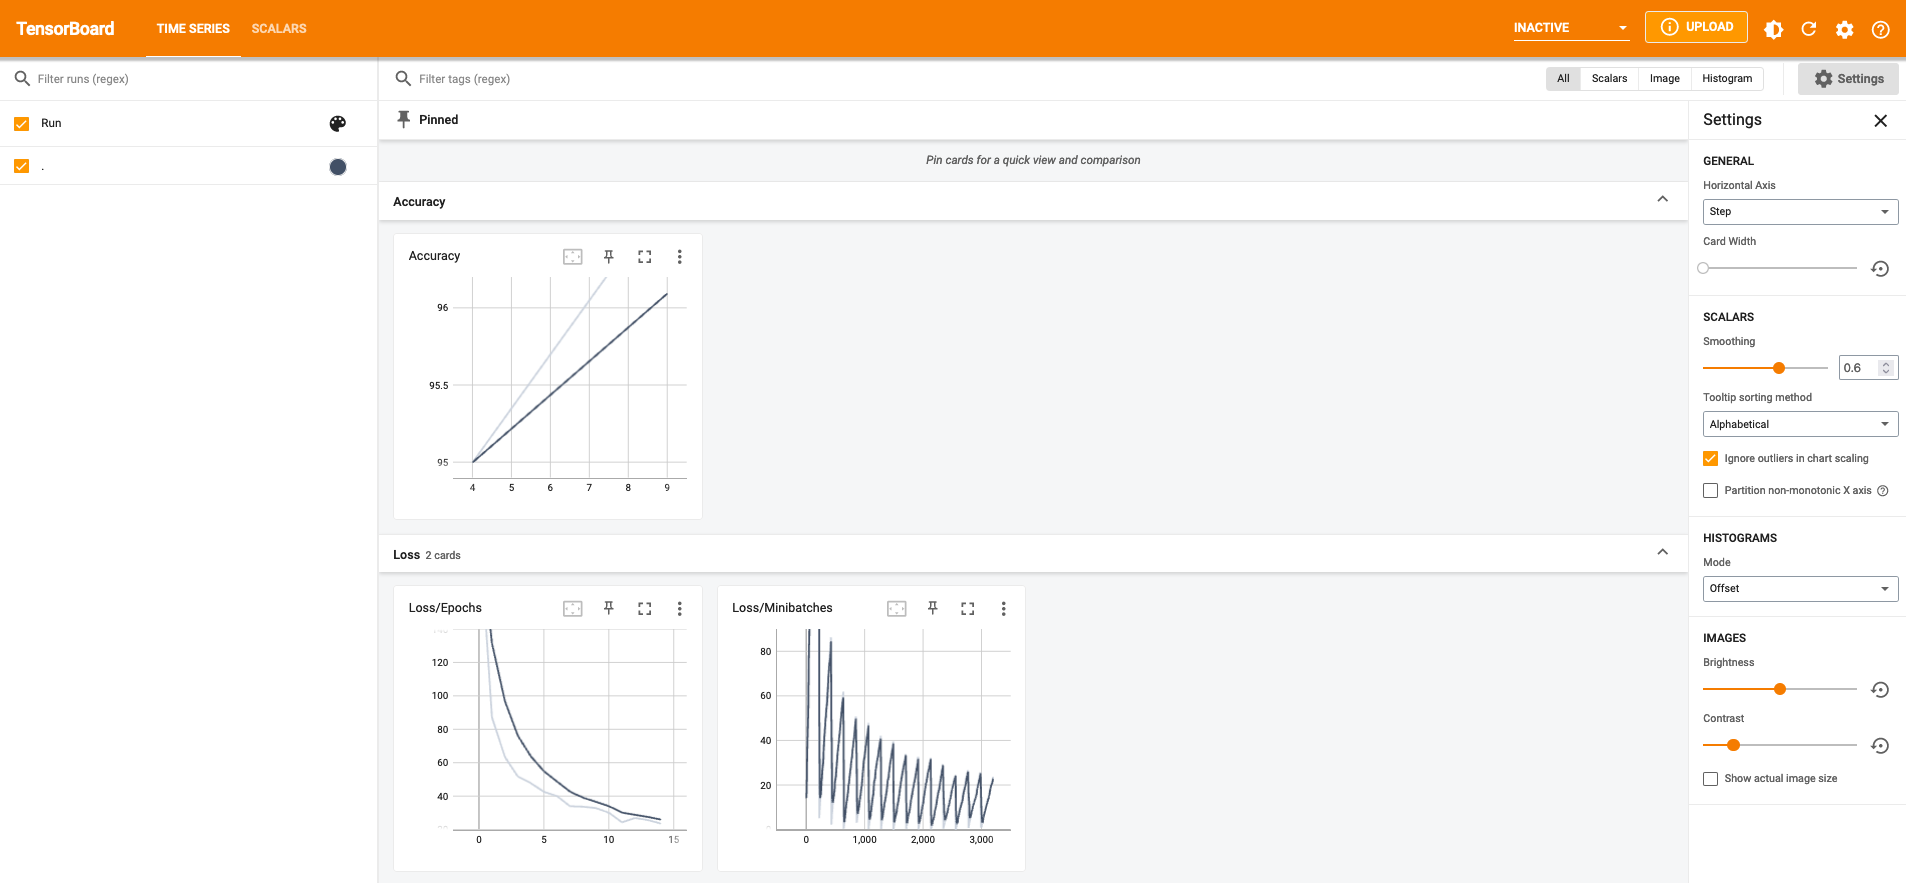
\includegraphics[width=1\textwidth]{./assets/scap_gtx1080_tensorboard_14615343}
\caption[TensorBoard - Accuracy and Loss]{TensorBoard - Accuracy and Loss for run 6 on the GTX 1080~(\Cref{tab:experiments-all})}
\label{fig:scap_gtx1080_tensorboard_14615343}
\end{figure}

\begin{figure}[H]
\centering
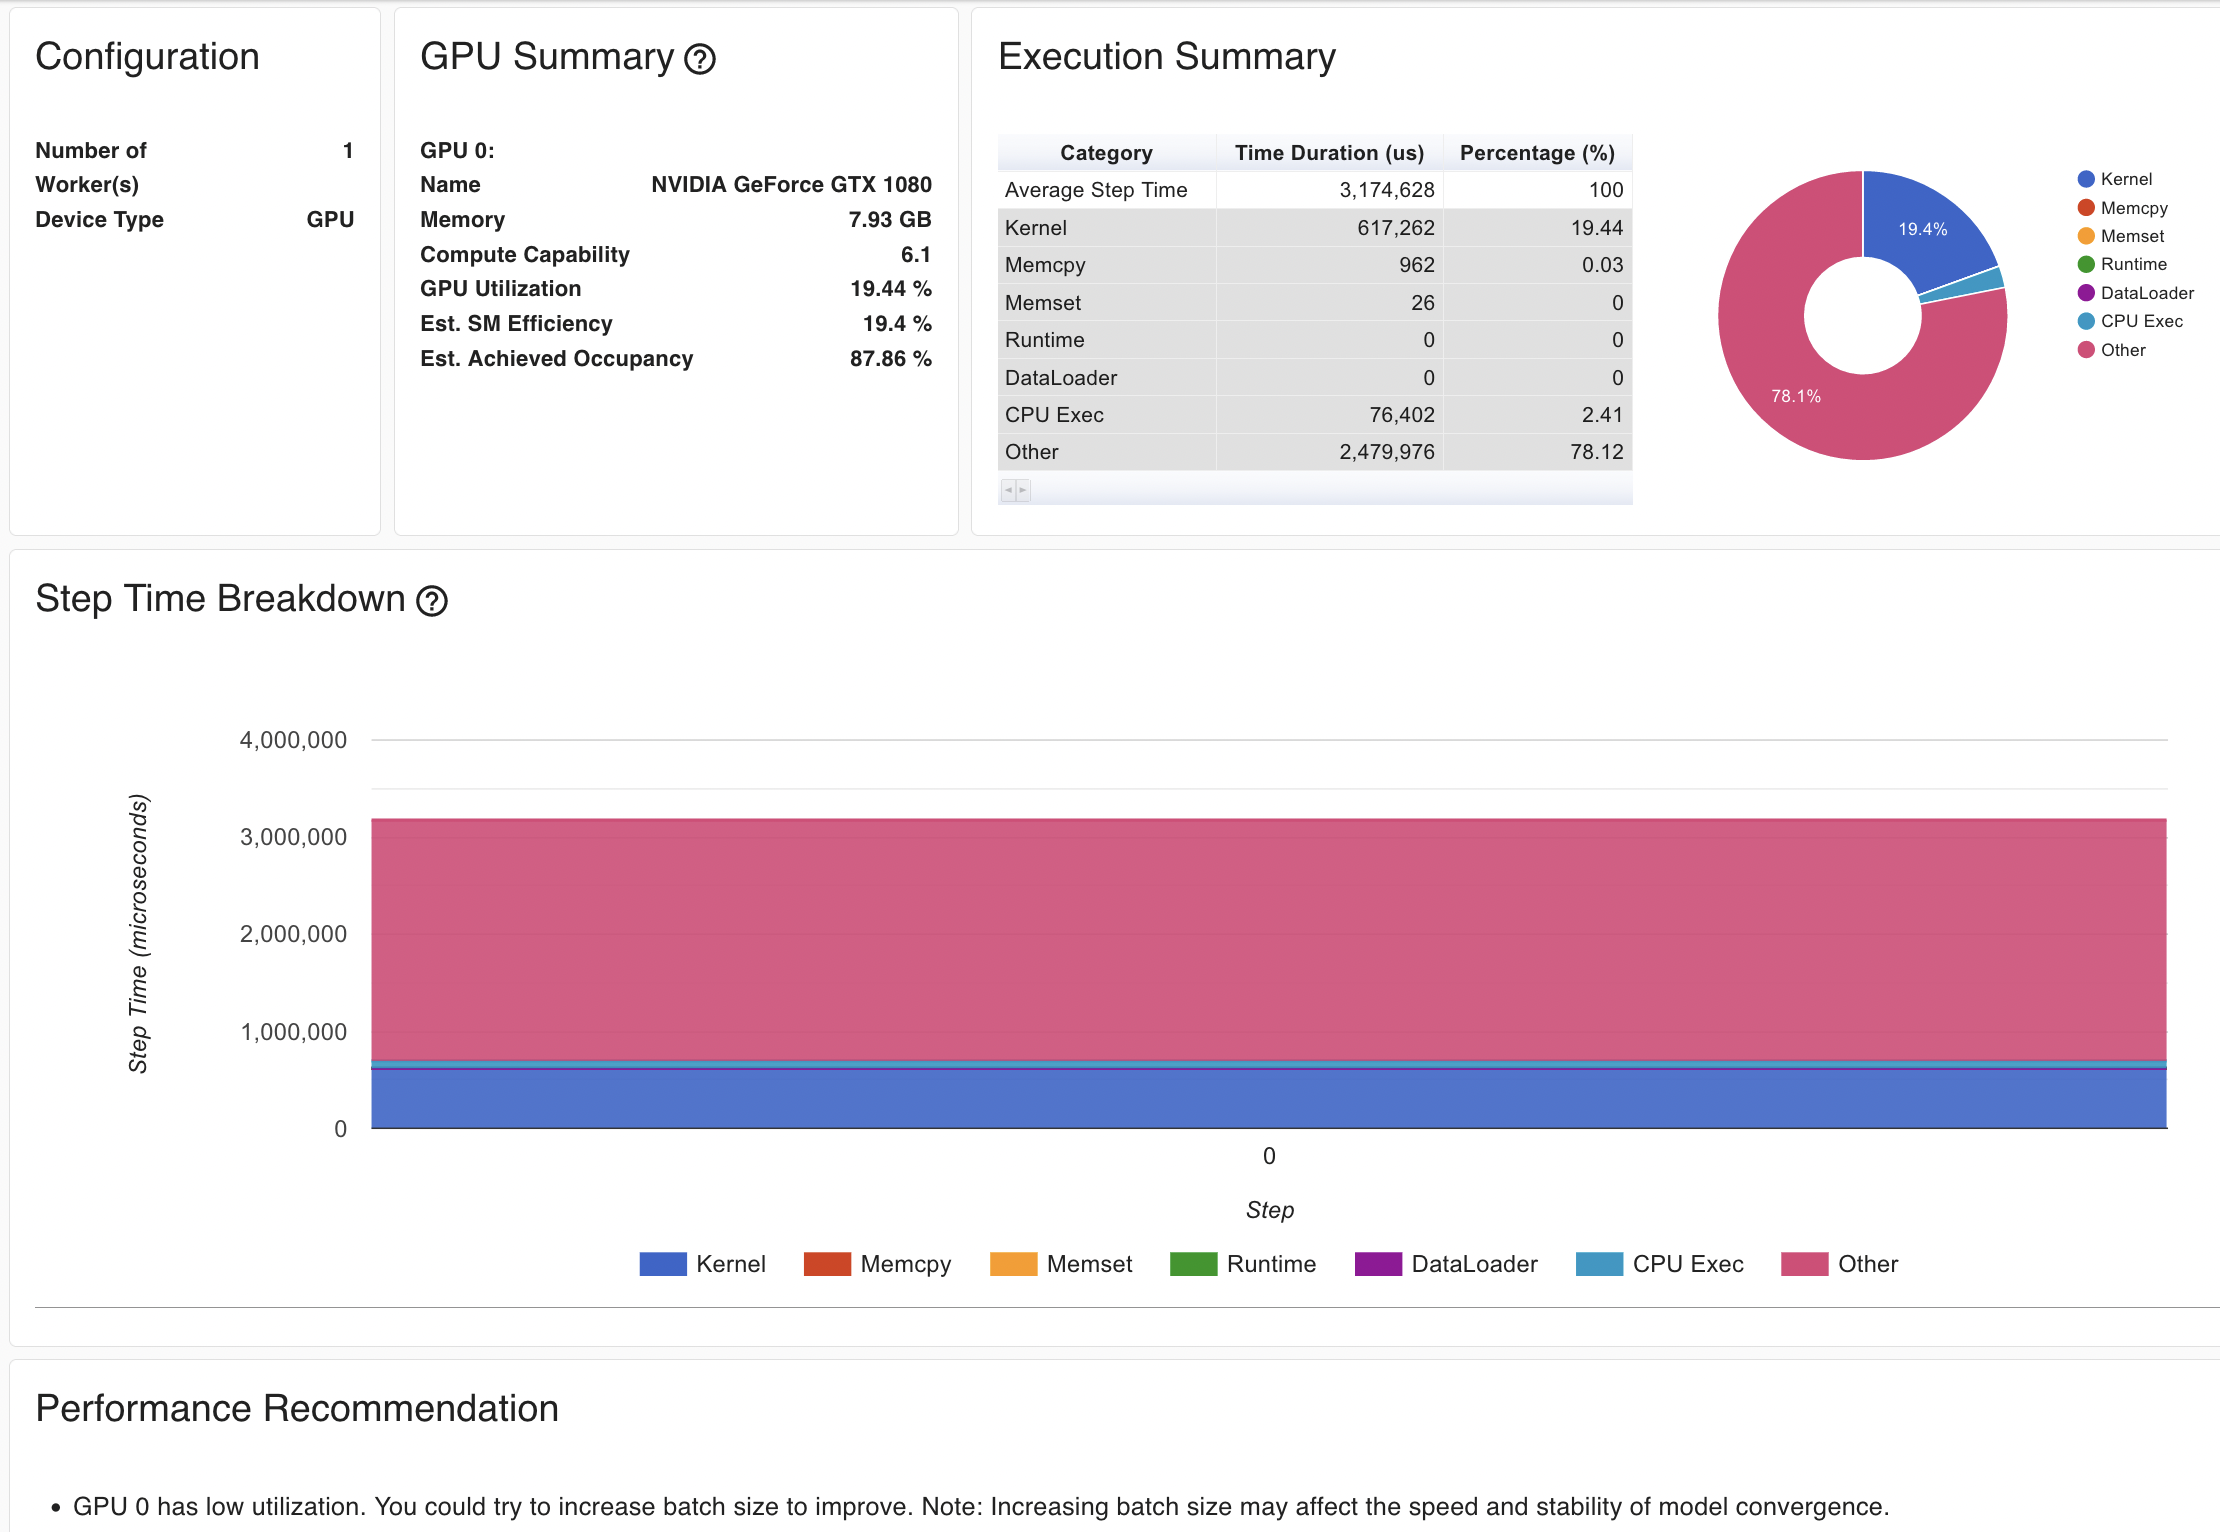
\includegraphics[width=1\textwidth]{./assets/scap_gtx1080_profiler-torch_batch-size-64_14650758}
\caption[PyTorch - Profiler: Overview - Increased batch size (64)]{PyTorch - Profiler: Overview - Increased batch size (64)}
\label{fig:scap_gtx1080_profiler-torch_batch-size-64_14650758}
\end{figure}

\begin{figure}[H]
\centering
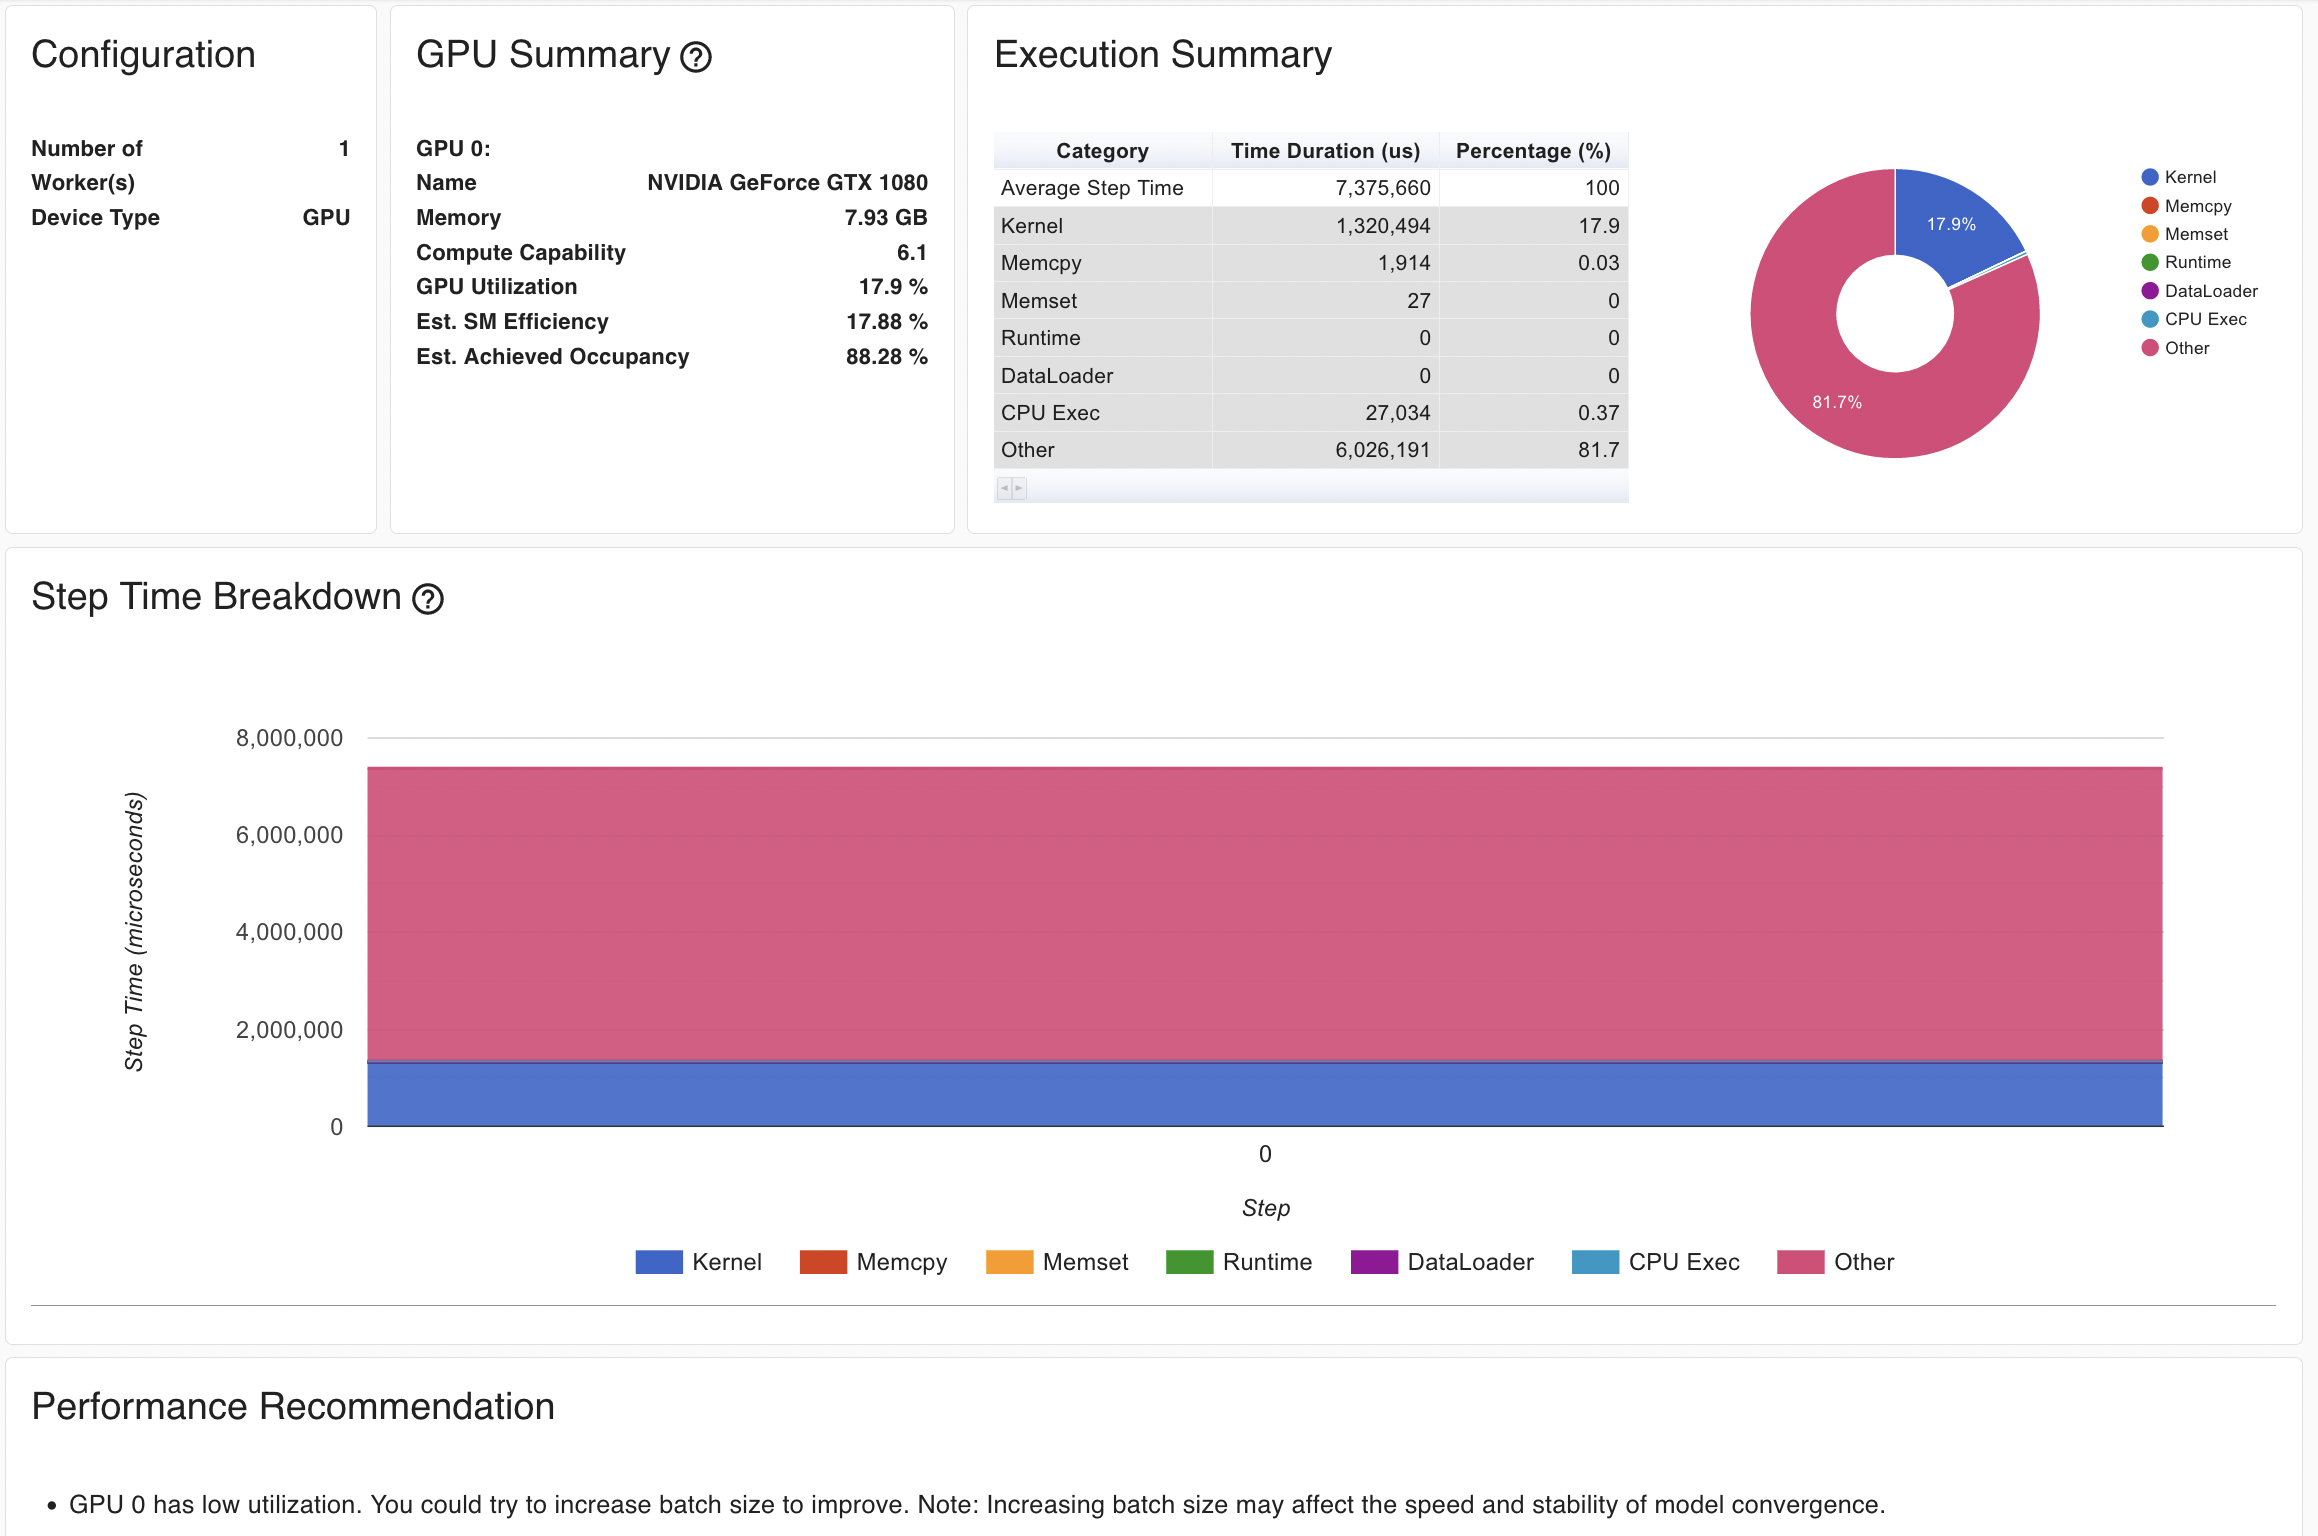
\includegraphics[width=1\textwidth]{./assets/scap_gtx1080_profiler-torch_batch-size-128_14650759}
\caption[PyTorch - Profiler: Overview - Increased batch size (128)]{PyTorch - Profiler: Overview - Increased batch size (128)}
\label{fig:scap_gtx1080_profiler-torch_batch-size-128_14650759}
\end{figure}

\begin{figure}[H]
\centering
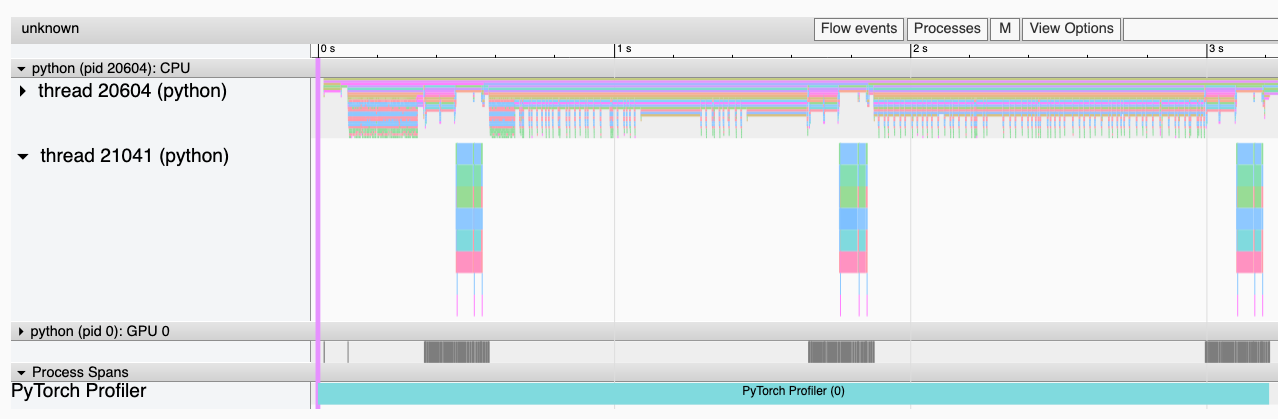
\includegraphics[width=1\textwidth]{./assets/scap_gtx1080_profiler-torch_batch-size-64_14650758_trace-view}
\caption[PyTorch - Profiler: Trace View]{PyTorch - Profiler: Trace View}
\label{fig:scap_gtx1080_profiler-torch_batch-size-64_14650758_trace-view}
\end{figure}

\begin{figure}[H]
\centering
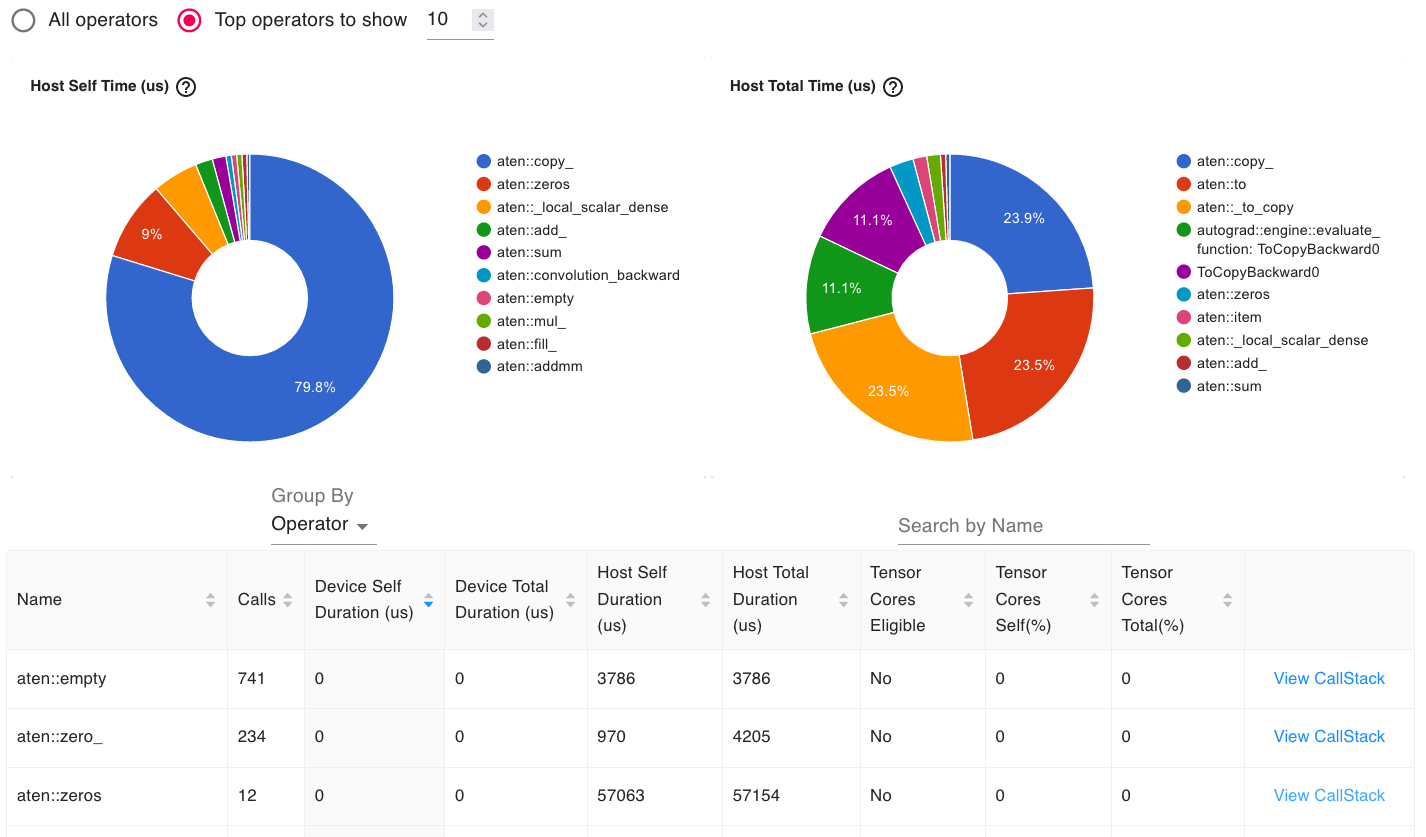
\includegraphics[width=0.9\textwidth]{./assets/scap_gtx1080_profiler-torch_batch-size-64_14650758_operator-view}
\caption[PyTorch - Profiler: Operator View]{PyTorch - Profiler: Operator View}
\label{fig:scap_gtx1080_profiler-torch_batch-size-64_14650758_operator-view}
\end{figure}

\begin{figure}[H]
\centering
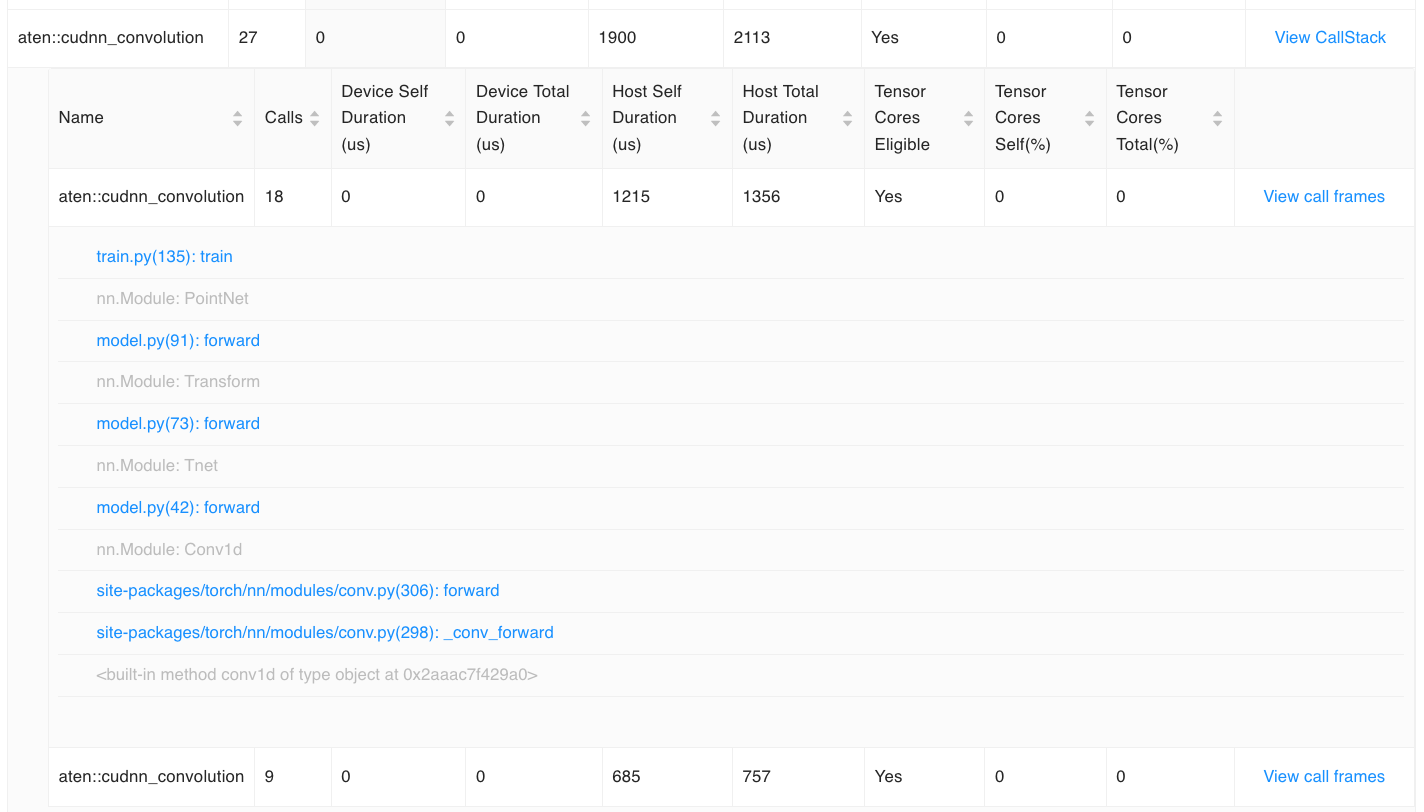
\includegraphics[width=0.9\textwidth]{./assets/scap_gtx1080_profiler-torch_batch-size-64_14650758_operator-view-details}
\caption[PyTorch - Profiler: Operator View (CallStack)]{PyTorch - Profiler: Operator View (CallStack)}
\label{fig:scap_gtx1080_profiler-torch_batch-size-64_14650758_operator-view-details}
\end{figure}

\begin{figure}[H]
\centering
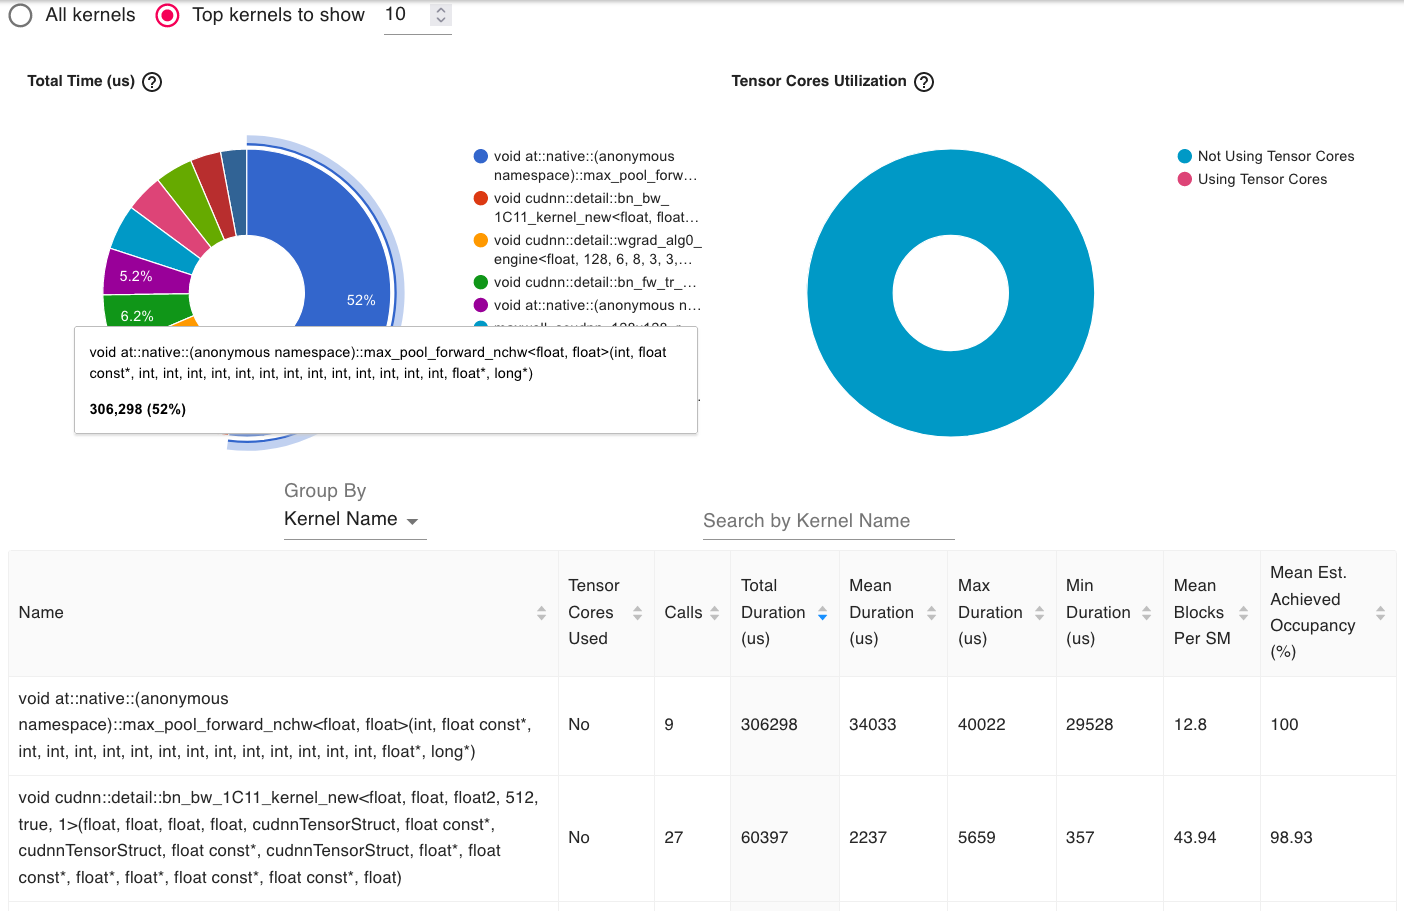
\includegraphics[width=0.9\textwidth]{./assets/scap_gtx1080_profiler-torch_batch-size-64_14650758_gpu-kernel-view}
\caption[PyTorch - Profiler: GPU Kernel View]{PyTorch - Profiler: GPU Kernel View}
\label{fig:scap_gtx1080_profiler-torch_batch-size-64_14650758_gpu-kernel-view}
\end{figure}

\begin{figure}[H]
\centering
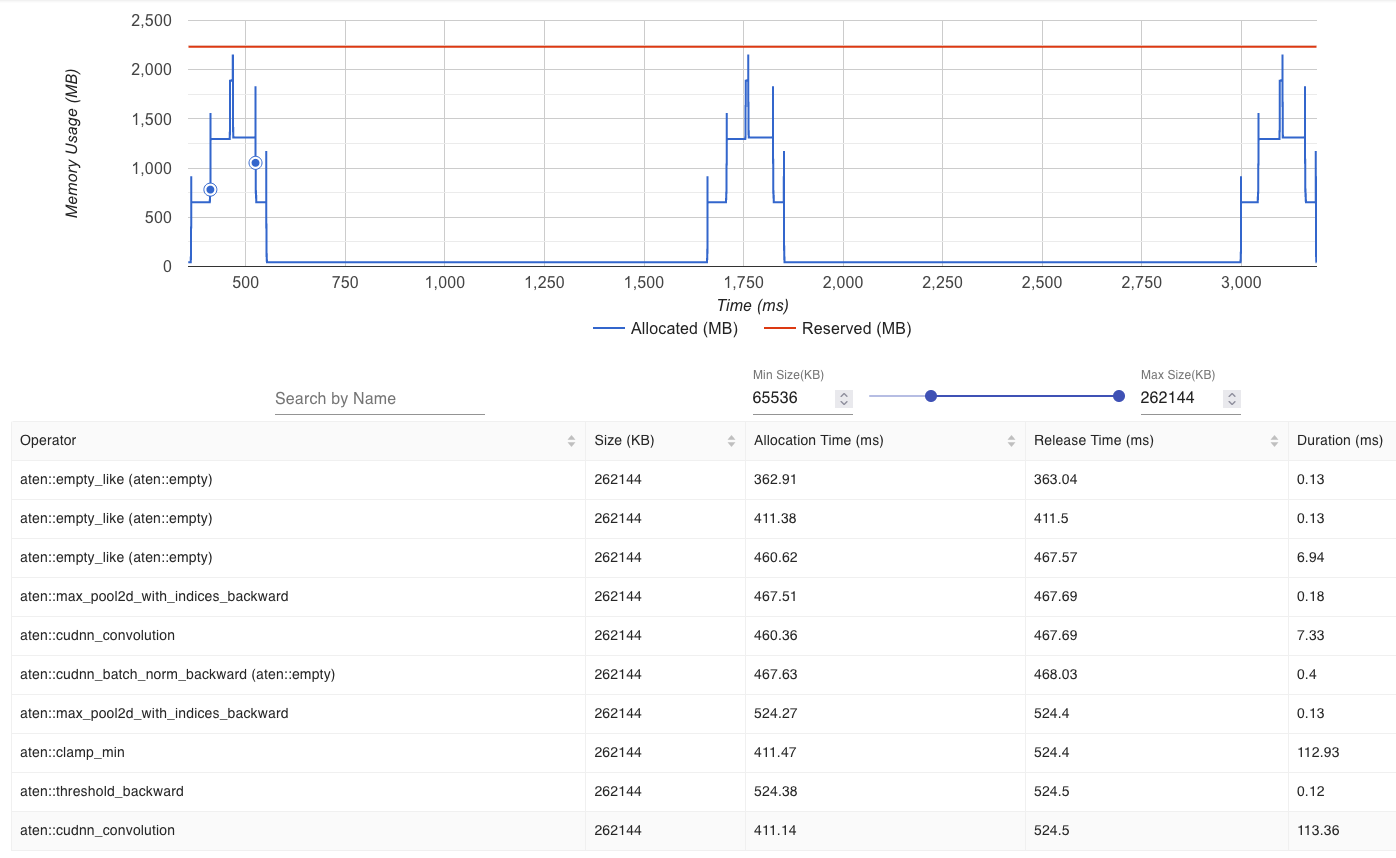
\includegraphics[width=0.85\textwidth]{./assets/scap_gtx1080_profiler-torch_batch-size-64_14650758_memory-view}
\caption[PyTorch - Profiler: Memory View]{PyTorch - Profiler: Memory View}
\label{fig:scap_gtx1080_profiler-torch_batch-size-64_14650758_memory-view}
\end{figure}

\begin{figure}[H]
\centering
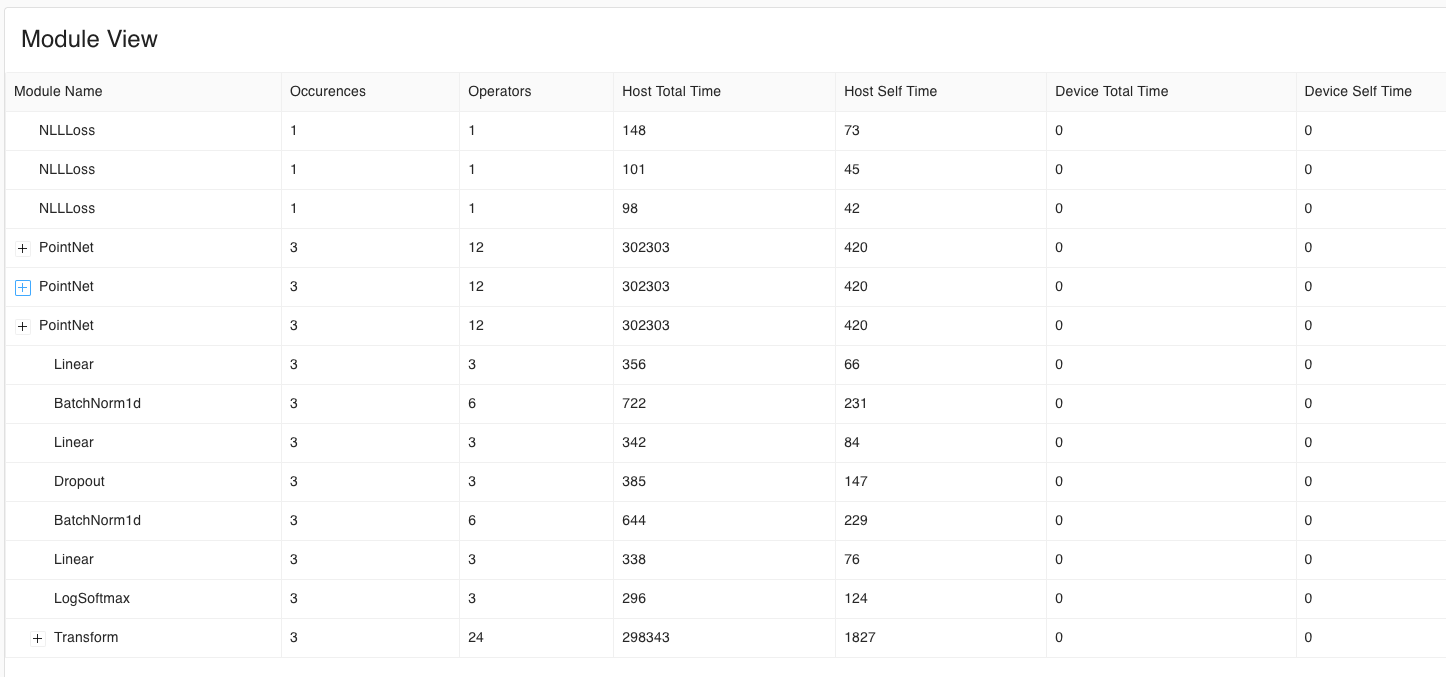
\includegraphics[width=1\textwidth]{./assets/scap_gtx1080_profiler-torch_batch-size-64_14650758_module-view}
\caption[PyTorch - Profiler: Module View]{PyTorch - Profiler: Module View}
\label{fig:scap_gtx1080_profiler-torch_batch-size-64_14650758_module-view}
\end{figure}

\inputminted[xleftmargin=1em,linenos,fontsize=\small, breaklines]{python}{./assets/scap_gtx1080_deepspeed_14615344_4294967294_one-epoch.txt}
\captionof{listing}{DeepSpeed - FlopProfiler: Full output\label{lst:scap_gtx1080_deepspeed_14615344_4294967294_one-epoch-full}}

\section{Code samples}

\begin{listing}[H]
\begin{minted}[breaklines]{python}
sacct --format=jobid,elapsed -P -j 14657599, 14617521, 14615343, 14650076, 14615344, 14617172, 14650079, 14617171, 14618941, 14617203, 14619619, 14650080, 14619618,14619617, 14617202, 14650750, 14650758, 14629421, 14629426, 14650740, 14650759 -X
        \end{minted}
\caption[Sacct command]{The command that is used to collect accounting information for the jobs executed on the \ac{SCC} for this project (\Cref{tab:experiments-all}). The output of this command can be found in~\Cref{lst:sacct_out}.}
\label{lst:sacct_command}
\end{listing}

\begin{listing}[H]
\inputminted[xleftmargin=1em,linenos,fontsize=\small, highlightlines={1,3,9-12,14-16}]{python}{./assets/tensorboard.py}
\caption[Code example for Tensorboard]{Highlighted parts of the code are required to use Tensorboard for profiling the training process of the neural network.}
\label{lst:tensorboard}
\end{listing}

\begin{listing}[H]
\inputminted[breaklines, xleftmargin=1em,linenos,fontsize=\small, highlightlines={4-10,14,15}]{python}{./assets/profiler-torch.py}
\caption[Code example for PyTorch - Profiler]{Highlighted parts of the code are required to use the PyTorch Profiler for profiling the training process of the neural network.}
\label{lst:profiler-torch}
\end{listing}

\begin{listing}[H]
\inputminted[xleftmargin=1em,linenos,fontsize=\small, highlightlines={1,3,4,8,9,11-18}]{python}{./assets/deepspeed.py}
\caption[Code example for Deepspeed - FLOPSProfiler]{Highlighted parts of the code are required to use Deepspeed - FLOPSProfiler for profiling the training process of the neural network.}
\label{lst:deepspeed}
\end{listing}

\end{document}  
